The Standard Model (\SM)~\cite{Peskin:257493} 
is a name given in the 1970s to a theory describing the fundamental particles and their interactions. This quantum field theory describes the particles and their interactions as fields and has successfully incorporated three of the four fundamental forces in the universe. In \Sec{sec:SMcontent}, the particle content of the \SM\ is summarised, while \Sec{sec:SMlagr} describes  the \SM\ Lagrangian and its symmetries. In \Sec{sec:FCNC}, the flavour content of the \SM\ is highlighted, and \Sec{sec:top} focusses on the top quark in the \SM.

The successful theory of the \SM\ has some shortcomings which are discussed in \Sec{sec:BSM} and lead to searches for a more general theory. One of such  is using  an effective field theory (EFT) approach~\cite{Burgess:2007pt}  to search for new physics in a model independent way.  A short introduction to the effective field theory approach is given in \Sec{sec:EFTSM}. In \Sec{sec:EFT}, an EFT model focussing on flavour changing neutral currents (FCNC) involving a top quark is presented. Its current experimental constraints are given in \Sec{sec:ExpConstr}.



\section{Elementary particles and forces}
\label{sec:SMcontent}
The interactions in nature can be described by four forces, the strong force, the electromagnetic (EM) force, the weak force and the gravitational force. These interactions happen via particles with an integer spin known as bosons. The strong interaction is mediated by eight gluons \Pgluon, while the electromagnetic force is mediated by photons \Pphoton, and the weak force by \PZ\ and \PWpm\ bosons. In \tab{tab:forces}, the forces and their characteristics are shown. The gravitational force is the only force not included in the \SM\ and can be neglected for energies lower than the Planck scale (1.22 $\times 10^{19}$~\GeV).
\begin{table}[htbp]
	\centering
	\caption{The four forces of nature and their characteristics.}
	\begin{tabular}{lcc}
		\toprule
		& Range & Mediator \\ 
		\midrule
		Strong force & $10^{-15}$ \m & 8 gluons  \\ 
	
		Electromagnetic force & $\infty$ & photon  \\ 
		 
		Weak force & $10^{-18}$ \m & \PWpm, \PZ\ bosons \\ 
		
		Gravitational force & $\infty$ & unknown \\ 
		\bottomrule
	\end{tabular} 
	\label{tab:forces}
\end{table}

The fermions are the particles that make up the visible matter in the universe. They carry half integer spin and can be subdivided into leptons and quarks, where leptons do not interact strongly. Each fermion has a corresponding anti-fermion which has the same mass and is oppositely charged. The electron \Pe\ is the first elementary particle discovered~\cite{electrondiscovery} and belongs to the first generation of leptons together with the electron neutrino \Pnue. The second generation comprises the muon \Pmu\ and muon neutrino \Pnum, whereas the third generation consists of the tau \Ptau\ and  tau neutrino \Pnut. The neutrinos are neutral particles, while the other leptons have charge $\pm \qe$ with \qe representing the elementary charge of 1.602~$\times 10^{-19}$~C. The masses of charged leptons differ by four orders of magnitude between the first and third generations. In the \SM\ the neutrinos are assumed to be massless, nonetheless it is experimentally established that neutrinos do have a tiny non-zero mass~~\cite{Fukuda:1998mi,PhysRevLett.108.131801}. In \tab{tab:leptongen}, the leptons and their properties in the \SM\ are summarised. 
\begin{table}[htbp]
	\centering
	\caption{The properties of the leptons in the three generations of the \SM~\cite{PDG}, where \qe represents the elementary  charge.}
	\begin{tabular}{lccc}
		\toprule
		Generation & Particle  & Mass  & Charge \\ 
		\midrule
		\multirow{2}{*}{First} & \Pelectron & 0.511~\MeV & $-\qe$  \\ 
		& \Pnue & $\approx$ 0 & 0\\
		
	\multirow{2}{*}{Second} & \Pmuon & 106~\MeV &$-\qe$  \\ 
	& \Pnum & $\approx$ 0 & 0\\
	
	\multirow{2}{*}{Third} & \Ptauon & 1777~\MeV & $-\qe$  \\ 
	& \Pnut & $\approx$ 0 & 0 \\
	
		
		\bottomrule
	\end{tabular} 
	\label{tab:leptongen}
\end{table}

The quarks are also divided into three generations. Unlike the leptons, they carry colour charge and can interact via the strong interaction. The top quark, discovered in 1995 at the Tevatron~\cite{observationtopD0,observationtopCDF}, is the heaviest \SM\ particle with a mass\footnote{In this thesis all masses and energies are expressed in natural units, where the speed of light and $\hbar$ are taken to be equal to one.} measured to be $173.34\pm0.27$(stat)$\pm0.71$(syst)~\GeV~\cite{ATLAS:2014wva}. The quarks and their properties are summarised in \tab{tab:quarkgen}. In nature, only colour neutral objects can exist. This has as consequence that quarks are bound through gluons into mesons (quark+anti-quark) and baryons (three quarks). These mesons and baryons are mostly short-lived and unstable particles that rapidly decay through \PWpm\ and \PZ\ bosons. The only known stable baryon is the proton, made up of two up quarks and one down quark.  
\begin{table}[htbp]
	\centering
	\caption{The properties of the quarks in the three generations of the \SM~\cite{PDG}, where \qe represents the elementary  charge.}
	\begin{tabular}{lccc}
		\toprule
		Generation & Particle  & Mass  & Charge \\ 
		\midrule
		\multirow{2}{*}{First} & up \Pup &$2.2_{-0.4}^{+0.6}$~\MeV& $\textfrac{2}{3}$ \qe  \\ [2.5mm]
		& down \Pdown & $4.7^{+0.5}_{-0.4}$ \MeV & $-\textfrac{1}{3}$ \qe\\[2.5mm]
		
		\multirow{2}{*}{Second} & charm \Pcharm & 1.28 $\pm$ 0.03~\GeV &$\textfrac{2}{3}$ \qe  \\ [2.5mm]
		& strange \Pstrange & $96^{+8}_{-4}$ \MeV & $-\textfrac{1}{3}$ \qe\\ [2.5mm]
		
		\multirow{2}{*}{Third} & top \Ptop & $173.34 \pm0.27$(stat)$\pm0.71$(syst)~\GeV &$\textfrac{2}{3}$ \qe  \\  [2.5mm]
		&bottom \Pbottom & $4.18^{+0.04}_{-0.03}$~\GeV & $-\textfrac{1}{3}$ \qe \\ [2.5mm]
		
		
		\bottomrule
	\end{tabular} 
	\label{tab:quarkgen}
\end{table}

The scalar boson, commonly known as the Higgs boson, is the last piece of the \SM\ discovered in 2012~\cite{Chatrchyan:2012xdj,Aad:2012tfa}. It is responsible for the masses of the \PWpm\ and \PZ\ boson, and that of the fermions.

\newpage
\section{Standard Model Lagrangian, connecting fields with particles}
\label{sec:SMlagr}
The \SM\ is a quantum field theory and thus describes the dynamics and kinematics of particles and forces by a Lagrangian \Lagr. The theory is based on the \SSU\ gauge symmetry, where \SU\ describes the electroweak interaction and \Sthree\ the strong interaction. The indices refer to colour C, the left chiral nature of the \Stwo\ coupling L, and the weak hypercharge Y. Its Lagrangian is constructed in a way that the symmetries representing physics conservation laws such as conservation of energy, momentum and angular momentum are represented. The symmetries under local gauge transformations are sustained by demanding gauge invariance\footnote{Different field configurations of unobservable fields can result in identical quantities. Transformations between such configurations are called gauge transformations and the absence of change in the measurable quantities is a characteristic called gauge invariance.}.  



The \Uone\ group has one generator Y with an associated gauge field \Bfield. The three gauge fields \Wfieldone, \Wfieldtwo, and \Wfieldthree, are associated to \Stwo\ with three generators that can  be written as half the Pauli matrices: 
\begin{equation}
T_1 =  \frac{1}{2}
\begin{pmatrix}
0  &  1      \\
1  & 0      
\end{pmatrix}, \;
T_2= \frac{1}{2}
\begin{pmatrix}
0  &  -i     \\
i  &  0      
\end{pmatrix},\;\mathrm{ and } \;
 T_3= \frac{1}{2}
 \begin{pmatrix}
 1  &  0     \\
 0  &  -1 
 \end{pmatrix}.
 \label{eq:Stwee}
\end{equation}
The generators $T^a$ satisfy the Lie algebra: 
\begin{equation}
 \left[T_a,T_b\right] = i \epsilon_{abc} T^c \; \mathrm{ and } \left[T_a, Y\right] = 0, 
\end{equation}
where $\epsilon_{abc}$ is an antisymmetric tensor. The gauge fields of \Stwo\ only couple to left-handed fermions as required by the observed parity violating nature of the weak force. The \Sthree\ group represents quantum chromodynamics (QCD). It  has eight generators corresponding to eight gluon fields \Gfields. Unlike \SU, \Sthree\ is not chiral. 

Under \Sthree, quarks are colour triplets while leptons are colour singlets. This implies that the quarks carry a colour index ranging between one and three, whereas leptons do not take part in strong interactions. Based on the chirality, the quarks and leptons are organized in doublets or singlets. Each generation $i$ of fermions consists of left-handed doublets and right-handed singlets: 
\begin{equation}
\mathrm{l}_{\mathrm{L,i}} =  
\begin{pmatrix}
\Pe_{\mathrm{L,i}}       \\
\Pneutrino_{\mathrm{L,i}}     
\end{pmatrix}, \; \Pe_{\mathrm{R,i}}, \; \mathrm{q}_{\mathrm{L,i}} = 
\begin{pmatrix}
\Pup_{\mathrm{L,i}}       \\
\Pdown_{\mathrm{L,i}}     
\end{pmatrix}, \; \Pup_{\mathrm{R,i}}, \; \mathrm{and} \; \Pdown_{\mathrm{R,i}}
\end{equation}

The \SM\ Lagrangian can be decomposed as a sum of four terms
\begin{equation}
\lagr_{\mathrm{SM}} = \lagr_{\mathrm{gauge}} + \lagr_{\mathrm{f}} + \lagr_{\mathrm{Yuk}} + \lagr_{\phi}, 
\end{equation}
that are related to the gauge, fermion, Yukawa and scalar sectors. The gauge Lagrangian regroups the gauge fields of all three symmetry groups, and the fermionic part consists of kinetic energy terms for quarks and leptons. The interaction between fermions and the scalar doublet $\phi$ gives rise to fermion masses and is described by the Yukawa Lagrangian. The scalar part of the Lagrangian is composed of a kinematic and potential component related to the scalar boson. 
%\begin{equation}
% \lagr_{\mathrm{gauge}} = -\frac{-1}{4} \Gtensord \Gtensoru -\frac{-1}{4} \Wtensord \Wtensoru - -\frac{-1}{4} \Btensord \Btensoru, 
%\end{equation}
%where the tensors are
%\begin{align}
%\Gtensord &= \partial_{\mu}\mathrm{G}_{\nu}^{\mathrm{i}} - \partial_{\nu}\mathrm{G}_{\mu}^{\mathrm{i}} - g_{\mathrm{s}} f_{ijk} \mathrm{G}_{\mu}^j \mathrm{G}_{\nu}^k, \; \mathrm{ with }\; i,j,k = 1,...,8 \\
%\Wtensord &= \partial_{\mu}\mathrm{W}_{\nu}^{\mathrm{i}} - \partial_{\nu}\mathrm{W}_{\mu}^{\mathrm{i}} - g_{\mathrm{s}} \epsilon_{ijk} \mathrm{W}_{\mu}^j \mathrm{G}_{\nu}^k, \; \mathrm{ with }\; i,j,k = 1,...,8 \\
%\end{align}

For the electroweak theory, two coupling constants are introduced, namely $g'$ for \Uone\ and $g$ for \Stwo. The physically observable gauge bosons of this theory are the photon field \photonfield, the \PZ\ boson field \Zfield, and the \PW\ boson fields \Wfield. These are a superposition of the four gauge fields of \SU: 
\begin{equation}
\begin{aligned}
\photonfield &= \sW \Wfieldthree + \cW \Bfield, \\
 \Zfield &= \cW \Wfieldthree - \sW \Bfield, \; \mathrm{ and } \\
  \Wfield &= \sqrt{\frac{1}{2}}\left(\Wfieldone\mp i \Wfieldtwo\right), 
\end{aligned}
\end{equation}
where $\theta_{\mathrm{W}}$ represents the weak mixing angle defined as $\mathrm{tan}\; \theta_{\mathrm{W}} = \frac{g'}{g}$.

The coupling constant representing the strength of the QCD interactions is denoted as $g_{\mathrm{s}}$. In QCD there is asymptotic freedom whereby the strong coupling constant becomes weaker as the energy with which the interaction between strongly interacting particles is probed increases, and stronger as the distance between the particles increases. A consequence of this is known as colour confinement, the quarks and gluons can not exist on their own and are not observed individually. They are bound in colour neutral states called hadrons, this process is known as hadronisation. 






\subsection*{Electroweak symmetry breaking}
In $\lagr_{\mathrm{gauge}}$ and $\lagr_{\mathrm{f}}$ are no mass terms for fermions present because only singlets under \SSU\ can acquire a mass with an interaction of the type $m^2\phi^{\dagger}\phi$ without breaking the gauge invariance. In order to accommodate mass terms for fermions and gauge fields, electroweak symmetry breaking leading to $\lagr_{\phi}$ is introduced. 

The scalar doublet is introduced in the \SM\ as 
\begin{equation}
\phi = \frac{1}{\sqrt{2}}
\begin{pmatrix}
\varphi_1 + i \varphi_2    \\
\varphi_3 + i \varphi_4    
\end{pmatrix}.
\end{equation}
Its field potential is of the form 
\begin{equation}
V(\phi) = \mu^2 \phi^{\dagger}\phi + \lambda(\phi^{\dagger}\phi)^2, 
\end{equation}
with $\mu^{2} <0$ and $\lambda$ a positive integer. This choice of parameters gives the potential a "Mexican hat" shape. It has an infinite set of minima (ground states) and by expanding the field around an arbitrary choice of ground state, the electroweak symmetry is broken (\cancel{EW}): 
\begin{equation}
\phi = 
\begin{pmatrix}
0    \\
\frac{v}{\sqrt{2}}    
\end{pmatrix}
+ \hat{\phi}, 
\end{equation}
where $v$ is the vacuum expectation value (vev), measured to be around 245~\GeV\ and corresponds to $\sqrt{\frac{-\mu}{\lambda}}$. The scalar doublet's four degrees of freedom are reduced to three degrees of freedom that couple to the gauge fields and fix the mass of the \PWp, \PWm\ and \PZ\ bosons. The remaining fourth degree of freedom has given rise to a physically observable particle, called the Brout-Englert-Higgs (BEH), \SM\ scalar or Higgs boson.
This spontaneous symmetry breaking leaves the gauge invariance intact and gives masses to the \PWpm\ and \PZ\ bosons as:
\begin{equation}
m_{\PW} = \frac{1}{2}v|g| \quad \mathrm{and} \quad m_{\PZ} = \frac{1}{2}v \sqrt{g'^2 + g^2}.
\end{equation}
The Higgs field couples universally to fermions with a strength proportional to their masses, and to gauge bosons with a strength proportional to the square of their masses. 


\section{Flavours in the \SM}
\label{sec:FCNC}
%In the electroweak theory, the \PW boson is responsible for flavour changing charged currents, and the \PZ boson for 
%lading W -> smamak veranderen -> niet voor Z , integendeel verboden op tree level onderdrukt op higher order
Flavour changing charged currents are introduced in 1963 by Nicola Cabibbo~\cite{PhysRevLett.10.531}. Via interactions with a \PW boson the flavour of the quarks is changed. At the time of the postulation only up, down,  and strange quarks were known and the charged weak current was described as a coupling between the up quark and $\Pdown_{\mathrm{weak}}$, where $\Pdown_{\mathrm{weak}}$ is a linear combination of the down and strange quarks, $\Pdown_{\mathrm{weak}}= \mathrm{cos }\:\theta_{\mathrm{c}} \:\Pdown + \mathrm{sin }\:\theta_{\mathrm{c}} \: \Pstrange$. This linear combination is a direct consequence of the chosen rotation
\begin{equation}
\begin{pmatrix}
\Pdown_{\mathrm{weak}} \\
\Pstrange_{\mathrm{weak}} 
\end{pmatrix}
 = 
 \begin{pmatrix}
 \mathrm{cos }\:\theta_{\mathrm{c}} &  \mathrm{sin }\:\theta_{\mathrm{c}} \\
 - \mathrm{sin }\:\theta_{\mathrm{c}} &  \mathrm{cos }\:\theta_{\mathrm{c}}
 \end{pmatrix}
 \begin{pmatrix}
 \Pdown \\
 \Pstrange 
 \end{pmatrix} = \mathcal{R} 
 \begin{pmatrix}
 \Pdown \\
 \Pstrange 
 \end{pmatrix}, 
\end{equation}
where the rotation angle $\theta_{\mathrm{c}}$ is known as the Cabibbo angle. This provides a definition for the charged weak current between \Pup\ and \Pdown\ quarks, 
\begin{equation}
J_{\mu} = \APup \gamma_{\mu}\left(1+\gamma_5\right)\Pdown_{\mathrm{weak}}. 
\end{equation} 
A consequence of Cabibbo's approach is that the $\Pstrange_{\mathrm{weak}}$ is left uncoupled, leading Glashow, Iliopoulos and Maiani (GIM)~\cite{PhysRevD.2.1285,BJORKEN1964255,Maiani:2013fpa} to require the existence of a fourth quark with charge $\textfrac{2}{3}\mathrm{q}_{\mathrm{e}}$. This quark, known as the charm quark, couples to $\Pstrange_{\mathrm{weak}}$ and the new definition of the charged weak current is
\begin{equation}
J_{\mu} = \begin{pmatrix}
\APup & \APcharm
\end{pmatrix}  \gamma_{\mu}\left(1+\gamma_5\right)\mathcal{R}  \begin{pmatrix}
d \\ s
\end{pmatrix}
\equiv \bar{U} \gamma_{\mu}\left(1+\gamma_5\right)\mathcal{R}D. 
\end{equation} 

The neutral weak current is defined as 
\begin{equation}
J_{3} = \bar{U} \gamma_{\mu}\left(1+\gamma_5\right)\left[\mathcal{R}, \mathcal{R}^{\dagger}\right]D, 
\end{equation} 
and is diagonal in flavour space. This has as consequence that no flavour changing neutral currents occur at tree-level interactions~\cite{Peskin:257493} in the \SM.


Kobayashi and Maskawa generalised the Cabibbo rotation matrix to accommodate a third generation of quarks. The result is a $3\times 3$ unitary matrix known as the CKM matrix $\mathcal{V}_{\mathrm{CKM}}$, responsible for the mixing of weak interaction states of down-type quarks: 
\begin{equation}
\begin{pmatrix}
\Pdown_{\mathrm{weak}} \\
\Pstrange_{\mathrm{weak}} \\
\Pbottom_{\mathrm{weak}}
\end{pmatrix}
= 
\begin{pmatrix}
V_{\Pup\Pdown} & V_{\Pup\Pstrange} & V_{\Pup\Pbottom} \\
V_{\Pcharm\Pdown} & V_{\Pcharm\Pstrange} & V_{\Pcharm\Pbottom} \\
V_{\Ptop\Pdown} & V_{\Ptop\Pstrange} & V_{\Ptop\Pbottom}
\end{pmatrix}
\begin{pmatrix}
\Pdown \\
\Pstrange \\
\Pbottom
\end{pmatrix} \equiv \mathcal{V}_{\mathrm{CKM}} \begin{pmatrix}
\Pdown \\
\Pstrange \\
\Pbottom
\end{pmatrix},
\end{equation}
where $\mathcal{V}_{\mathrm{CKM}}$ is unitary $\left(\mathcal{V}_{\mathrm{CKM}}^{\dagger}\mathcal{V}_{\mathrm{CKM}} = \mathbb{1}\right)$. A general $3\times 3$ unitary matrix depends on three real angles and six phases. For the CKM matrix, the freedom to redefine the phases of the quark eigenstates can remove fives of the phases, leaving a single physical phase known as the Kobayashi-Maskawa phase. This phase is responsible for the charge parity violation in the \SM~\cite{CKM}. 
% see wolfenstein parametrisation http://pdg.lbl.gov/2017/reviews/rpp2016-rev-cp-violation.pdf 13,53
Each element $|V_{\mathrm{ij}}|$ of $ \mathcal{V}_{\mathrm{CKM}}$ squared represents the transition probability of a quark i going to a quark j, and is experimentally determined to be~\cite{PDG}
\begin{equation}
\mathcal{V}_{\mathrm{CKM}} =
\begin{pmatrix}
0.97425 \pm 0.00022  & 0.2253 \pm 0.0008      & (4.13 \pm 0.49) \times 10^{-3} \\
0.225 \pm 0.008      & 0.986 \pm 0.016        & (41.1 \pm 1.3) \times 10^{-3} \\
(8.4\pm 0.6) \times 10^{-3} & (40.0 \pm 2.7) \;10^{-3} & 1.021 \pm 0.032
\end{pmatrix}.
\label{eq:CKM}
\end{equation}

From  \eq{eq:CKM} follows that top quarks predominantly decay via charged weak currents to bottom quarks, with a probability consistent with unity. In the \SM, FCNC can only occur via higher loop interactions which are highly suppressed. The expected transition probabilities for a top quark decaying via a FCNC interaction in the \SM\ are given in \tab{tab:FCNCBR}, where it is clear that the FCNC top quark interactions of the \SM\ are still beyond the reach of the sensitivity of current experiments. 
\begin{table}[htbp]
	\centering
	\caption{The predicted branching fractions \BR\ for FCNC decays involving the top quark in the \SM~\cite{AguilarSaavedra:2004wm}.}
	\begin{tabular}{lc|lc}
		\toprule
	    Process	& \BR\ in the \SM  &  Process	& \BR\ in the \SM \\ 
		\midrule
		$ \Ptop \rightarrow \Pup \PZ $         & $8  \times 10^{-17}$  &	$ \Ptop \rightarrow \Pcharm \PZ $      & $1  \times 10^{-14}$   \\
		$ \Ptop \rightarrow \Pup \Pphoton $    & $4  \times 10^{-16}$  & $ \Ptop \rightarrow \Pcharm \Pphoton $ & $5  \times 10^{-14}$   \\
		$ \Ptop \rightarrow \Pup \Pgluon $     & $4  \times 10^{-14}$  & $ \Ptop \rightarrow \Pcharm \Pgluon $  & $5  \times 10^{-12}$  \\
		$ \Ptop \rightarrow \Pup \PHiggs $     & $2  \times 10^{-17}$  & $ \Ptop \rightarrow \Pcharm \PHiggs $  & $3  \times 10^{-15}$ \\
		\bottomrule
	\end{tabular} 
	\label{tab:FCNCBR}
\end{table}

\newpage
\section{The top quark in the \SM}
\label{sec:top}
\label{sec:TopSM}
Discovered in 1995 by the CDF and D0 collaborations at the Tevatron with proton-antiproton data~\cite{Abachi:1995iq,Abe:1995hr,}, the top quark plays an important role in  high energy physics. Its Yukawa interaction is given by
\begin{equation}
\lagr_{\mathrm{top-Yukawa}} = -\frac{\lambda_t v}{\sqrt{2}} \APtop_{\mathrm{L}} \Ptop_{\mathrm{R}} -\frac{\lambda_{\Ptop} }{\sqrt{2}} \PHiggs\ \APtop_{\mathrm{L}} \Ptop_{\mathrm{R}} + \mathrm{h.c.},
\end{equation}
yielding a Yukawa coupling of~\cite{PDG}
\begin{equation}
 \lambda_{\mathrm{t}} = \frac{\sqrt{2}m_{\Ptop}}{v} = 0.991 \pm 0.003.
\end{equation}
 This Yukawa coupling is very large compared to the other Yukawa couplings in the SM (\order$(10^{-2})$), leading to the belief that the top quark may have an important role in understanding the mechanism of electroweak symmetry breaking. On top of this, the very short lifetime of the top quark makes it an excellent candidate to study the properties of a bare quark. Its high mass, almost 40 times higher than the mass of the closest fermion in mass, leads to a large coupling with the Higgs boson and makes the top quark an interesting candidate to investigate how particles acquire mass. 


The CKM matrix element $V_{\Ptop\Pbottom}$, given in \eq{eq:CKM}, is experimentally found to be much larger than $V_{\Ptop\Pstrange}$, $V_{\Ptop\Pdown}$, and close to unity. The top quark decays through electroweak interactions since the  \PW\ boson mass is smaller than the top quark mass and the \PW\ boson can be on shell. A consequence of this is that the top quark has a very short lifetime of only $1/\Gamma_{\Ptop}\approx 5 \: 10^{-25}$~\s~\cite{PDG} leading to the fact that the formation of bound states involving top quarks is not allowed. This lifetime is even shorter than the typical hadronisation timescale of $1/\Lambda_{\mathrm{QCD}}\approx 10^{-23}$ \s, prohibiting gluons to radiate from the top quark and keeping its spin coherent. Since the electroweak interactions have a vector-axial vector (V-A) coupling structure\footnote{In the \SM\ a vector - axial vector coupling structure $\left(\gamma^{\mu} - \gamma^{\mu}\gamma^5\right)$ is predicted  that only permits left-handed fermions  or right-handed anti fermions to interact with a spin-1 particle. }
%\footnote{For an interaction where a spin-1 particle is exchanged, the most general form is a linear combination of a vector and an axial vector. From experiments, the weak interaction is determined to have this V-A structure: $J^{\mu} \prop \APup_{\Pneutrino}\left(\gamma^{\mu} - \gamma^{\mu}\gamma^5\right)\Pup_{\Pe}$.}
, the top quark spin orientation can be derived from the angular distributions of its decay products. This makes it possible to study the polarisation of top quarks from the angular distributions in various processes. 


The massiveness of the top quark leads to the fact that a large amount of energy is needed to create one. This is only the case for high energy collisions such as those happening in the Earth's upper atmosphere when cosmic rays collide with particles in air, or by particle accelerators. The production of top quarks happens in two ways: single via the electroweak interaction or in pairs via the strong interaction. At hadron colliders, the dominant production mechanism is top quark pair production via gluon (gg$\rightarrow$\ttbar) or quark fusion (\qqbar $\rightarrow$ \ttbar). In \fig{fig:toppairproduction}, the different top quark pair production mechanisms are shown. The production channel of gluon fusion is the main contributor to the top quark pair cross section at the LHC compared to quark fusion at the Tevatron. % because of the increasing gluon PDF towards smaller momentum fraction
The gg$\rightarrow$\ttbar\ process contributes 80-90\% to the total top quark pair cross section in the LHC centre-of-mass energy regime of 7-14~\TeV~\cite{PDG}. In \tab{tab:toppaircros} the predicted top quark pair production cross sections are given for the LHC and the Tevatron, while in \fig{fig:ttcross}, a summary plot of the LHC and Tevatron top quark pair cross section measurements as a function of the centre-of-mass energy can be found. These measurements are found to be in agreement with their \SM\ predictions. 
%\begin{figure}[htbp]
%	\centering
%	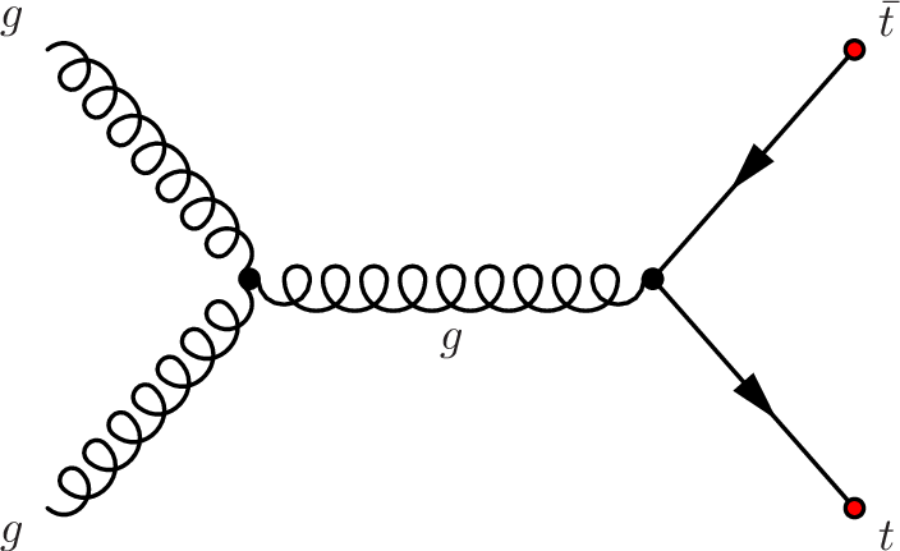
\includegraphics[width=0.32\linewidth]{1_Introduction/Figures/Ttbar_production_via_gg_fusion}
%	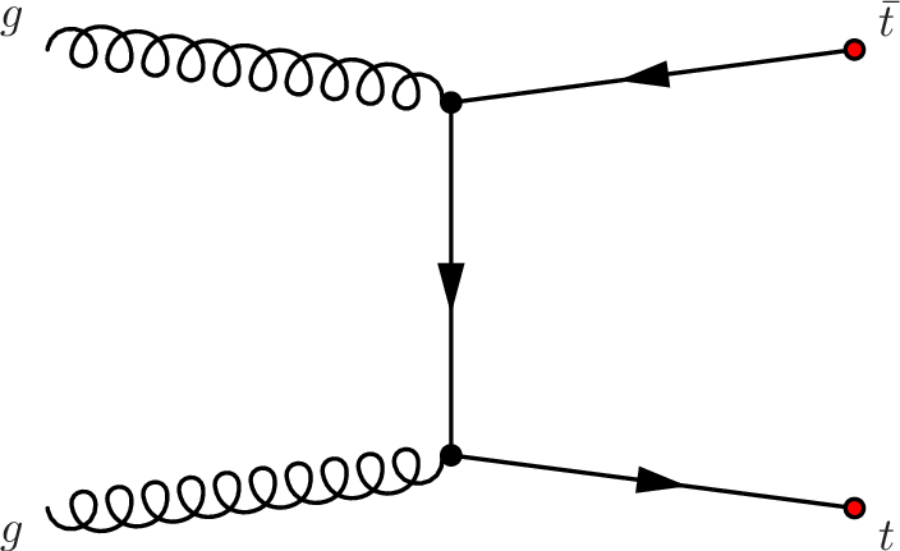
\includegraphics[width=0.32\linewidth]{1_Introduction/Figures/Ttbar_production_(t_channel)}
%	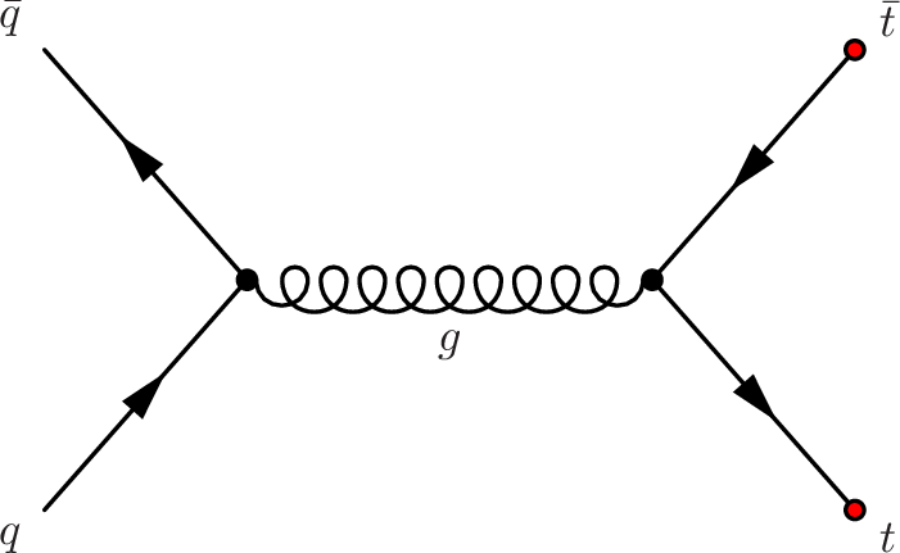
\includegraphics[width=0.32\linewidth]{1_Introduction/Figures/Ttbar_production_via_qqbar_annihilation}
%	\caption{Leading order diagrams of the top quark pair production. Gluon fusion (left and middle)are the dominant processes at the LHC, while quark fusion (right) is the dominant one at Tevatron. }
%	\label{fig:toppairproduction}
%\end{figure}
\begin{figure}[htbp]
	\centering
	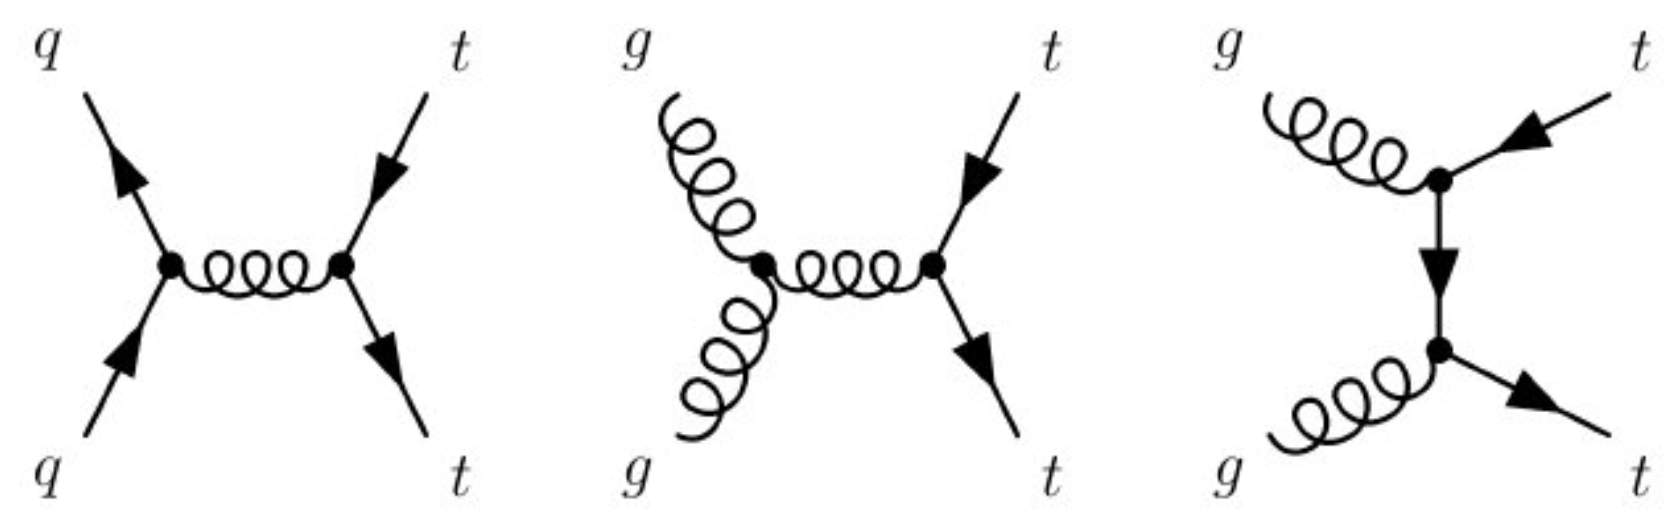
\includegraphics[width=0.7\linewidth]{1_Introduction/Figures/toppair}
	\caption{Leading order diagrams of the top quark pair production. Gluon fusion (right and middle) are the dominant processes at the LHC, while quark fusion (left) is the dominant one at the Tevatron. }
	\label{fig:toppairproduction}
\end{figure}
\begin{table}[htbp]
	\centering
	\caption{Predictions on the top quark pair production cross sections at next-to-next-to-leading order per centre-of-mass energy~\cite{PDG}. The first uncertainty is from scale dependence, while the second uncertainty originates from parton density functions.}
	\begin{tabular}{llll}
		\toprule
	 Experiment & Top quark mass &Centre-of-mass energy& Cross section (\pb) \\ 
		\midrule
		Tevatron & $m_{\Ptop} = 173.3 \:~\GeV$ & $\sqrt{s} = 1.96$~\TeV & $\sigma_{\ttbar} = 7.16^{+0.11+0.17}_{-0.20-0.12}$  \\ [2.5mm] 
		LHC & $m_{\Ptop} = 173.2~\GeV$ & $\sqrt{s} = 7$~\TeV & $\sigma_{\ttbar} =173.6^{+4.5+8.9}_{-5.9-8.9}$  \\ [2.5mm]
		LHC & $m_{\Ptop} = 173.2~\GeV$ & $\sqrt{s} = 8$~\TeV & $\sigma_{\ttbar} =247.7^{+6.3+11.5}_{-8.5-11.5}$  \\ [2.5mm]
		LHC & $m_{\Ptop} = 173.2~\GeV$ & $\sqrt{s} = 13$~\TeV & $\sigma_{\ttbar} =816.0^{+19.4+34.4}_{-28.6-34.4}$  \\ [2.5mm]
	\bottomrule
	%http://pdg.lbl.gov/2017/reviews/rpp2016-rev-top-quark.pdf
	\end{tabular} 
	\label{tab:toppaircros}
\end{table}

\begin{figure}[htbp]
	\centering
	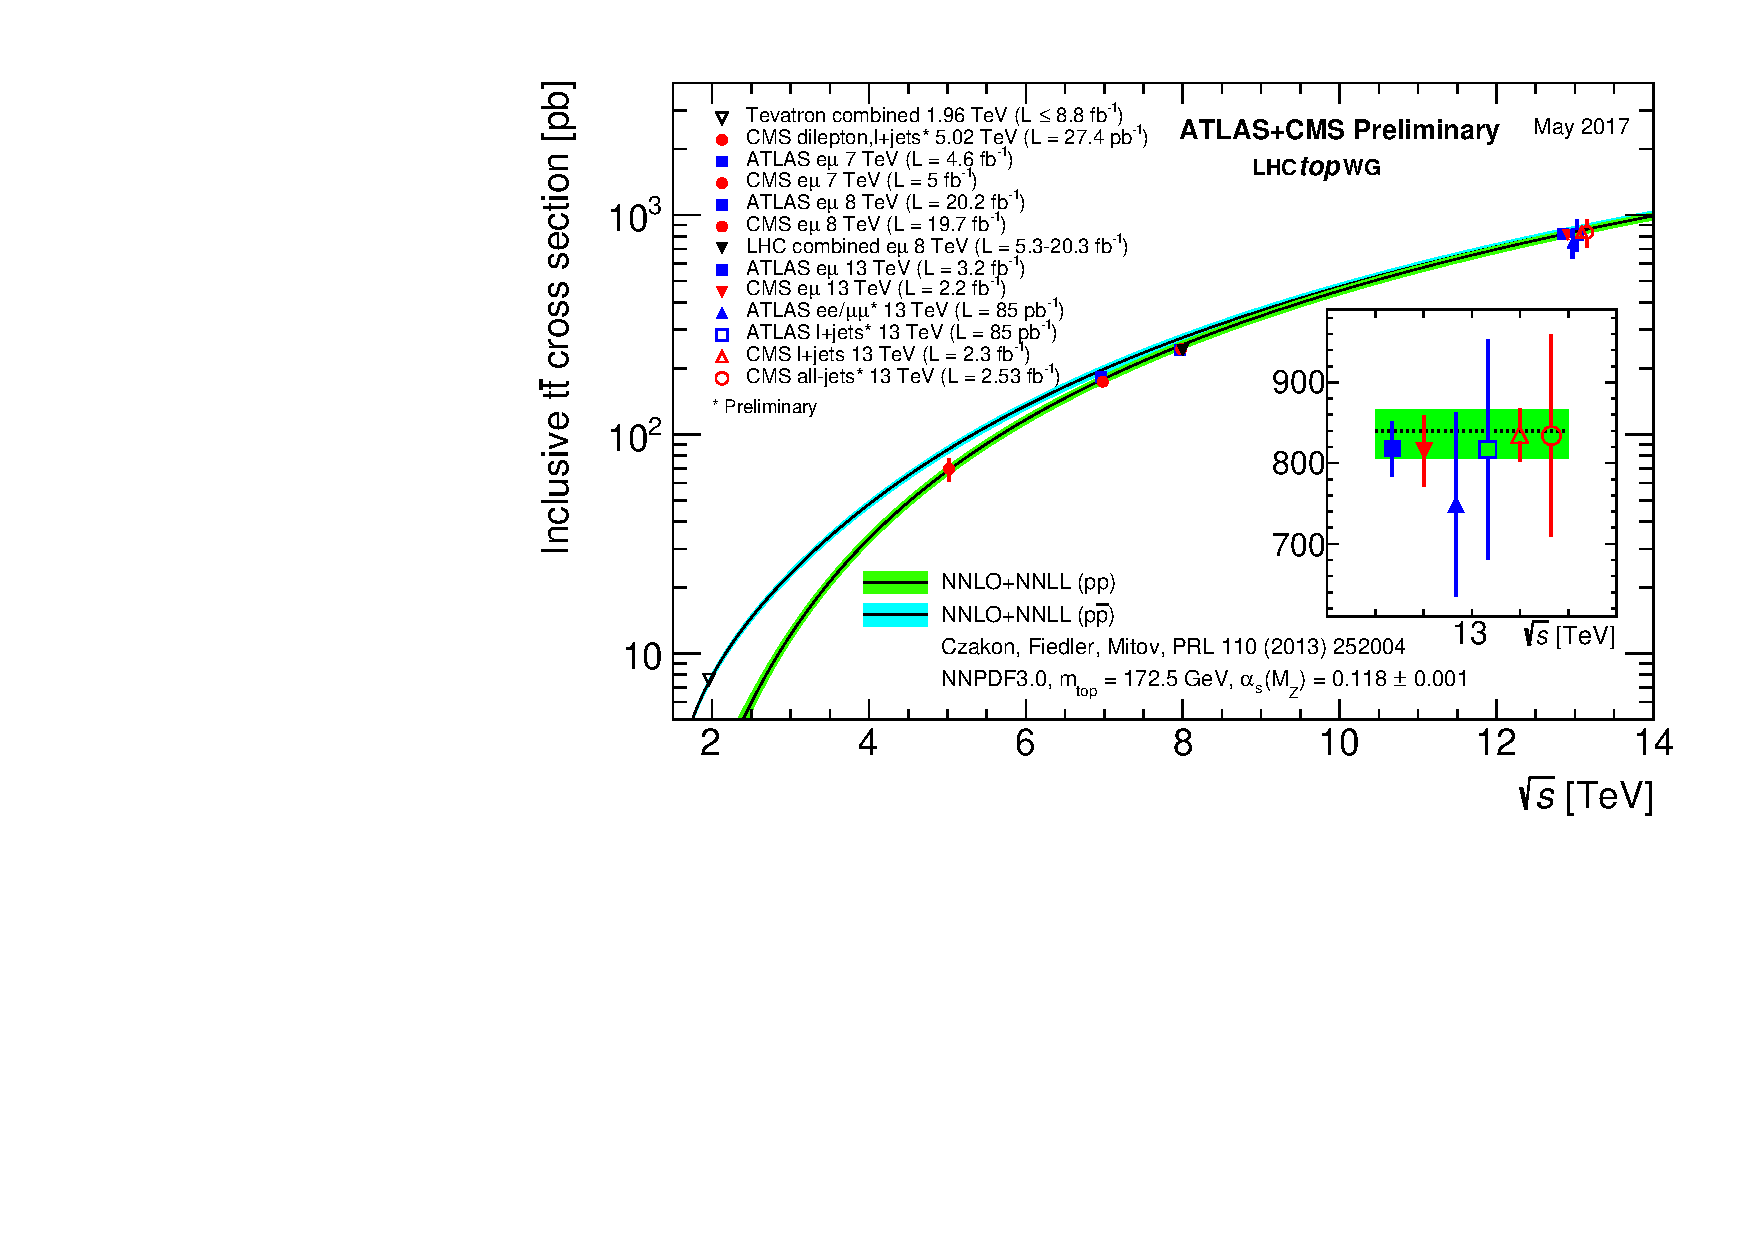
\includegraphics[width=1.\linewidth]{1_Introduction/Figures/tt_xsec_vsroots.pdf}
	\caption{Summary of the LHC and the Tevatron measurements of the top quark pair production cross section as function of the centre-of-mass energy compared with the next-to-next-to-leading order QCD calculation. The theory bands are the uncertainties due to renormalization and factorisation scales, parton density functions and the strong coupling. The mass of the top quark is assumed to be 172.5~\GeV. Measurements for the same centre-of-mass energy are slightly off-set for clarity.  Figure taken from \cite{summarytwiki}.}
		\label{fig:ttcross}
\end{figure}

The singly produced top quarks are produced via the electroweak interaction. These production mechanisms are subdivided at leading order into three main channels based on the virtuality ($Q^2 = - p_{\mu}p^{\mu}$) of the exchanged \PW\ boson. In \fig{fig:singletop}, the corresponding Feynman diagrams are shown. The single top quark production cross sections, given in \tab{tab:singletopcros}, are smaller than the top quark pair production cross sections since the electroweak coupling strength is smaller than the strong coupling strength. In addition, for the single top quark production, there is the need of sea quarks (\Pbottom, \APquark) in the initial states for which the parton density functions increase less steeply at low momentum fractions compared to the gluon parton density functions. 
\begin{comment}
	Electroweak single top-quark production mechanisms, na- mely from qq′ → tb [4], qb → q′t [5], mediated by virtual s-channel and t-channel W-bosons, and Wt-associated pro- duction, through bg → W−t, lead to somewhat smaller cross sections. For example, t-channel production, while suppressed by the weak coupling with respect to the strong pair produc- tion, is kinematically enhanced, resulting in a sizable cross section both at Tevatron and LHC energies. At the Tevatron, the t- and s-channel cross sections of top and antitop are identical, while at the LHC they are not, due to the charge- asymmetric initial state. 
\end{comment}
\begin{figure}[htbp]
	\centering
	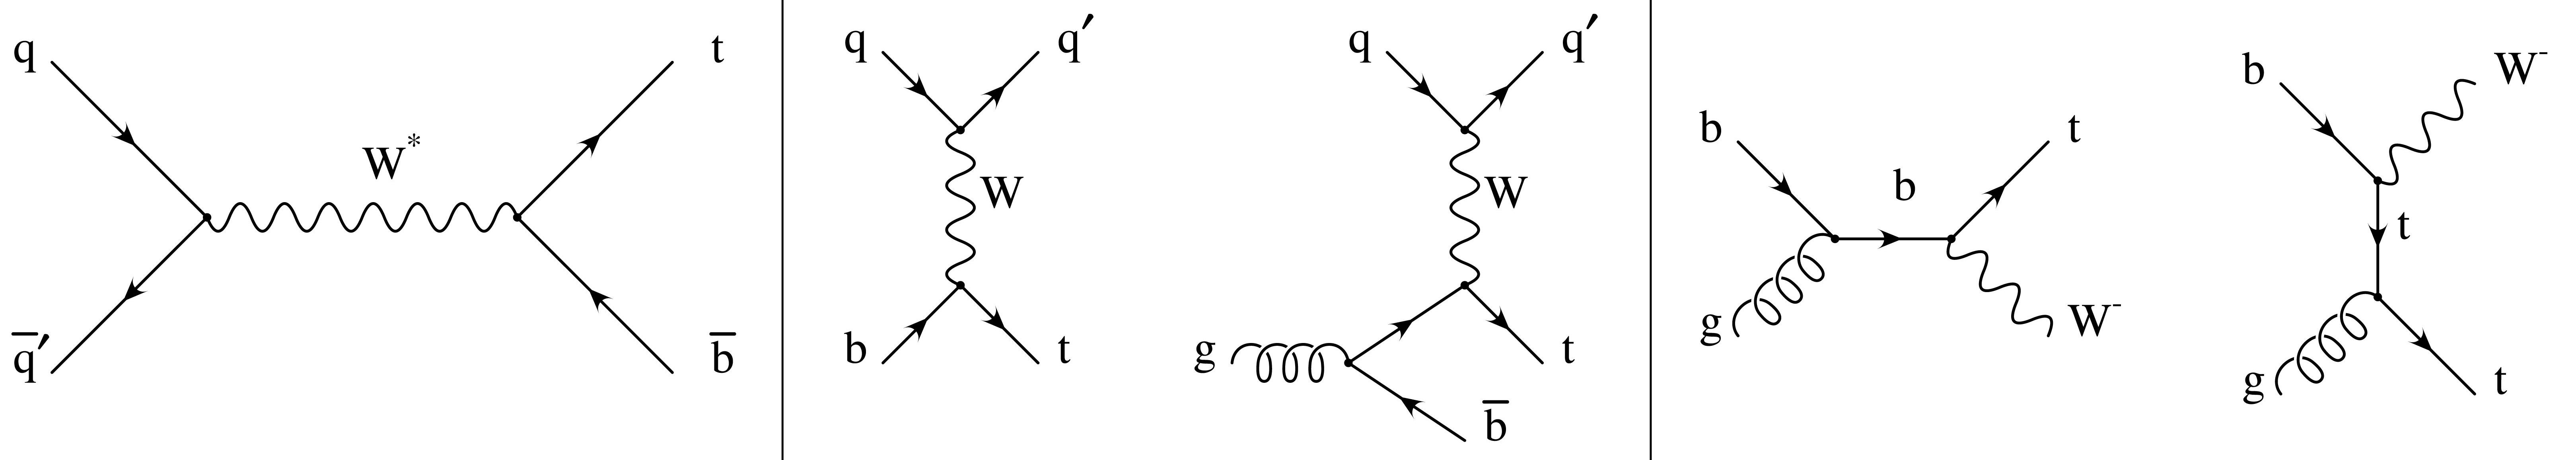
\includegraphics[width=1.\linewidth]{1_Introduction/Figures/single_Top_channels_0}
	\caption{Leading order Feynman diagrams of the electroweak production of single top quarks in the $s$-channel (left), $t$-channel (middle), and for the tW associated production. Figure taken from \cite{singletop}.}
	\label{fig:singletop}
\end{figure}

The production via the $t$-channel has a virtuality of the \PW\ boson $Q^2>0$, making it space-like. It is produced via the scattering of the \PW\ boson of a bottom quark coming from a proton or from gluon splitting (\Pgluon$\rightarrow$\bbbar). It has the highest single top quark cross section in proton collisions and the top quark production is roughly twice as large than the antitop quark. This is a consequence of the up-down valence quark composition of the proton. This feature makes the $t$-channel sensitive to the parton density functions of the proton. %The ratio depends however on the center-of-mass energy since at higher energies lower momentum fractions are probed at which contributions from the valence quarks become less dominant.
The $s$-channel is the production mechanism with the smallest cross section. Here the \PW\ boson is time-like ($Q^2 <0$) which requires the \PW\ boson to have a large virtuality to produce the heavier top quark. It is produced from two quarks belonging to the same isodoublet (e.g. \Pup\APdown) and subsequently decays to \Ptop\APbottom. This process gets enhanced by many beyond the Standard Model scenarios via the addition of new heavy particles such as \PW'. The tW-channel has a top quark produced in association with a \PW\ boson produced on shell, $Q^2 = -m^2_{\PW}$. This mode is negligible at the Tevatron, but of relevant size at the LHC. The tW-channel is sensitive to new physics affecting the Wtb vertex.  The single top quark production cross section measurements by the CMS collaboration can be found in \fig{fig:stcross} and are not showing any significant deviations from their \SM\ predictions.
 
 \begin{table}[htbp]
 	\centering
 	\caption{Predictions on the single top quark production cross sections at next-to-leading order per centre-of-mass energy~\cite{PDG}. The  uncertainties from scale dependence and from parton density functions are combined in quadrature or given separately (scale + PDF). For the $t$-channel the relative proportions to \Ptop\ and \APtop\ are 65\% and 35\%. For the $s$-channel this is respectively 69\% and 31\%. The tW-channel has an equal proportion of top and antitop quarks. For Tevatron, the top quark mass is assumed to be 173.3~\GeV, while the LHC predictions use $m_{\Ptop} = 172.5$~\GeV~\cite{PDG,stwiki}.} 
 	\begin{tabular}{lllll}
 		\toprule
 		Collider & Centre-of-mass energy& \multicolumn{3}{c}{Cross section $\sigma_{\Ptop+\APtop}$ (\pb)} \\ 
 		                     &                     &  $t$-channel & $s$-channel & tW-channel \\
 		\midrule
 		{Tevatron} & {$\sqrt{s} = 1.96$~\TeV }& $ 2.06^{+0.13}_{-0.13}$ &$  1.03^{+0.05}_{-0.05}$  & $-$ \\  [2.5mm]
 		                        
 		{LHC} &{ $\sqrt{s} = 7$~\TeV }& $ 63.89^{+2.91}_{-2.52}$ &$  4.29^{+0.19}_{-0.17}$  & $ 15.74^{+0.40+1.10}_{-0.40-1.14}$ \\  [2.5mm]
 		{LHC} & { $\sqrt{s} = 8$~\TeV} & $ 84.69^{+3.76}_{-3.23}$ &$  5.24^{+0.22}_{-0.20}$  &  $ 22.37^{+0.60+1.40}_{-0.60-1.40}$  \\ [2.5mm]
 		{LHC} &  {$\sqrt{s} = 13$~\TeV }& $ 216.99^{+9.04}_{-7.71}$ &$  10.32^{+0.40}_{-0.36}$  &  $ 71.7^{+1.80+3.40}_{-1.80-3.40}$  \\ [2.5mm] 
 		\bottomrule
 		%http://pdg.lbl.gov/2017/reviews/rpp2016-rev-top-quark.pdf
 		%https://twiki.cern.ch/twiki/bin/view/LHCPhysics/SingleTopRefXsec#Predictions_at_7_8_13_and_14_TeV
 	\end{tabular} 
 	\label{tab:singletopcros}
 \end{table}

\begin{figure}[htbp]
	\centering
	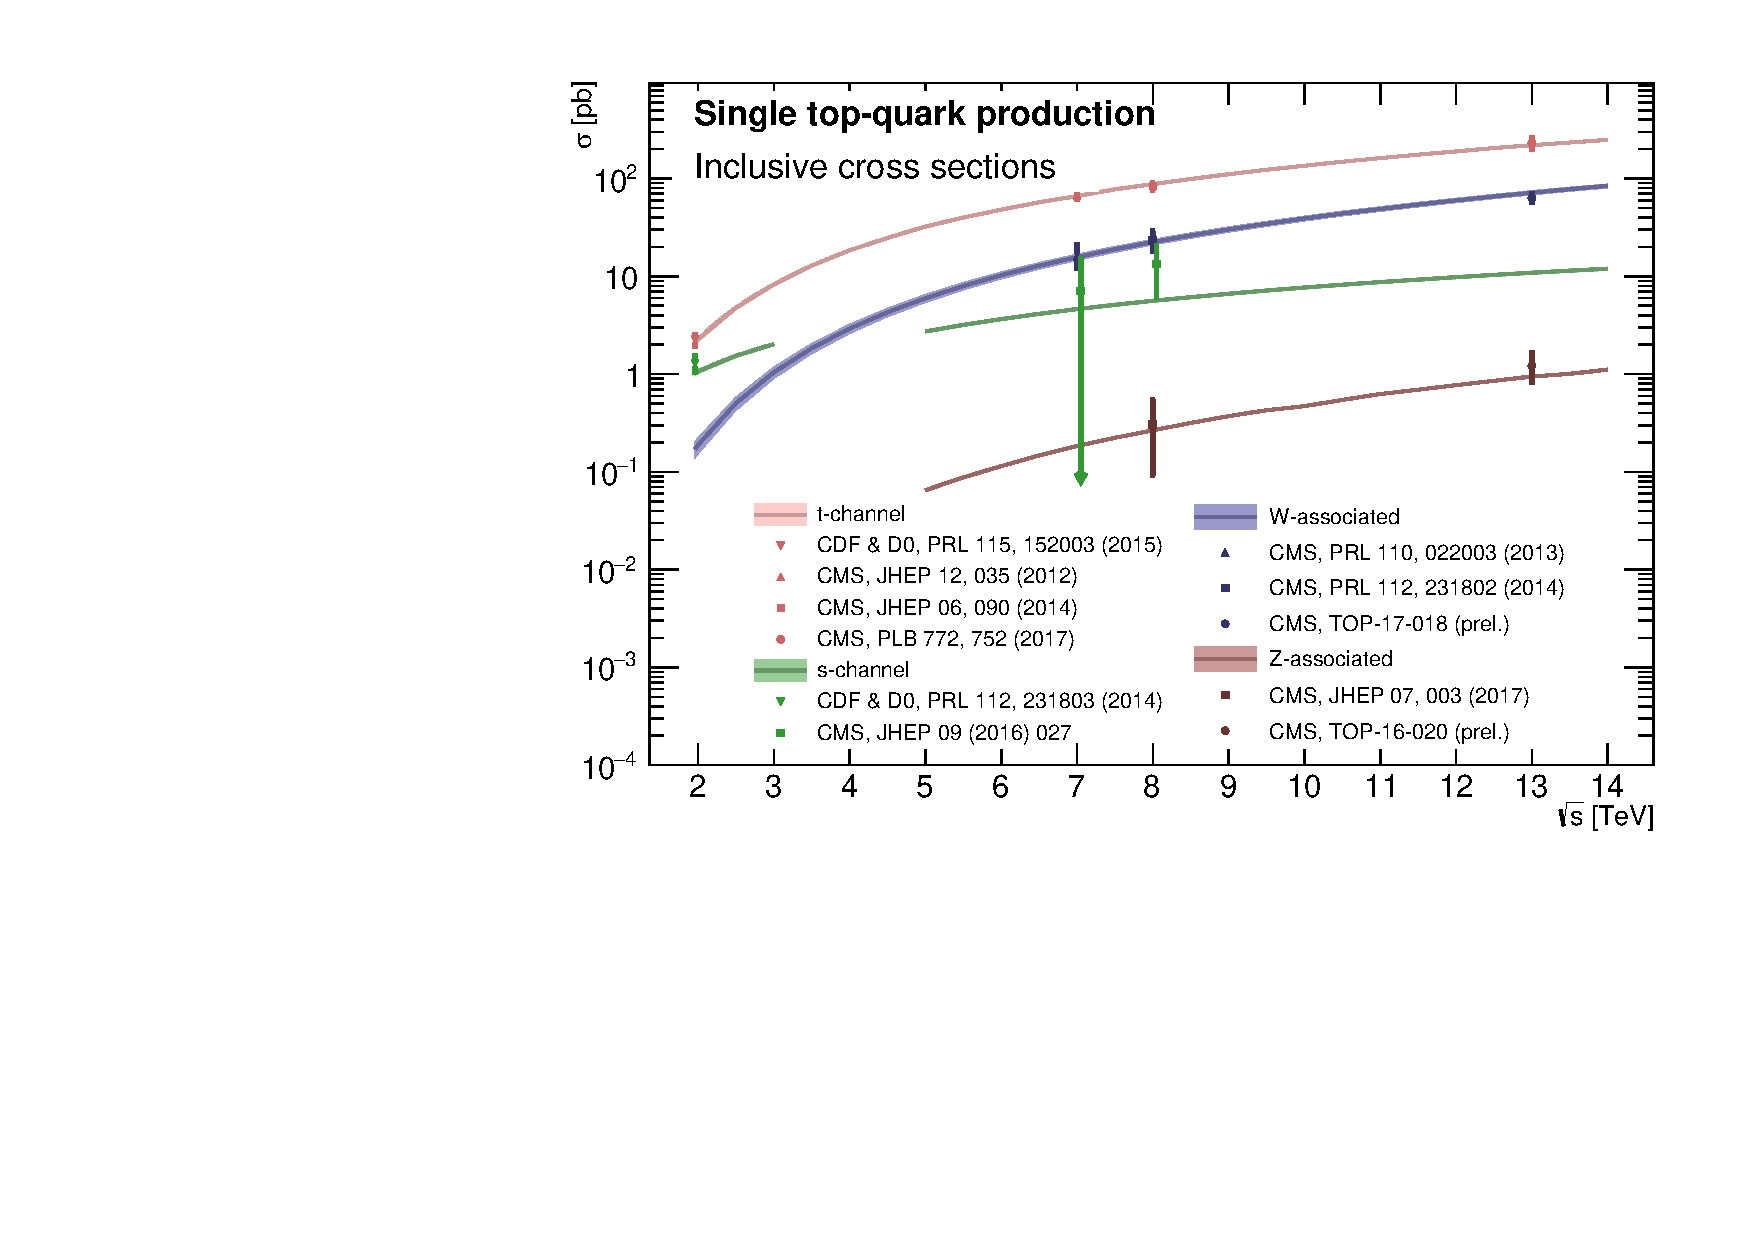
\includegraphics[width=1.\linewidth]{1_Introduction/Figures/singletop_sqrts.pdf}
	\caption{Summary of the measurements of the single top top quark production cross section as function of the centre-of-mass energy. Figure taken from \cite{summarywiki}.}
	\label{fig:stcross}
\end{figure}

\section{Effective field theories}
\label{sec:EFTSM}
%https://cp3.irmp.ucl.ac.be/upload/theses/phd/degrande.pdf
%http://www.physi.uni-heidelberg.de/Forschung/he/LHCb/documents/WorkshopNeckarzMarz08/TF_OPE.pdf
Problems can be simplified if one looks at the relevant scale of the process that one want to investigate, for example the chemical properties of an hydrogen atom can be described without any knowledge of quark interactions inside the proton. In this case, the proton can be considered the elementary object (indivisible) due to the fact that the binding energy of the constituents is much bigger than the energy of the electron in orbit around the proton. Effective field theories are based on this kind of separation of different energy scales in a system~\cite{thesisDeg}. Effective field theories can be used for theories where the perturbative expansion cannot be trusted, e.g. QCD at low energy, or as bottom up approach to look for new physics in a model independent way. The latter is the way effective field theory will be used throughout this thesis. 


The main idea behind effective field theory is easily explained via the example of the Fermi theory. Fermi explained in 1933~\cite{Fermi2008} the $\beta$-decay as a product of currents: 
\begin{equation}
\Lagr^{\mathrm{Fermi}}_{\mathrm{EFT}} = - \frac{G_{\mathrm{F}}}{\sqrt{2}} J^{\mu}J_{\mu}^{\dagger},
\label{eq:EFTfermi}
\end{equation}
where $G_{\mathrm{F}}$ is the Fermi coupling constant, measured to be $G_{\mathrm{F}} \approx 1.17 \times 10^{-5}~\GeV^{-2}$. The current $J_{\mu}$ can written as the sum of an hadronic $J_{\mu}^h$ and leptonic $J_{\mu}^l$ current, where for simplicity only the leptonic current is discussed. 
\begin{equation}
	J_{\mu}^l = \sum \limits_{\mathrm{l}} \APnu_{\mathrm{l}} \gamma_{\mu} \left(1-\gamma_5\right) \mathrm{l}.
\end{equation}
Historically, charged currents were flavour universal and the later discovered parity violation of the weak interaction led to the V-A structure. After this, the \Stwo\ symmetry was postulated and the existence of neutral currents was predicted. The effective Lagrangian used then (given in \eq{eq:EFTfermi}), could nowadays be build starting from \Stwo\ symmetries only. 

The muon decay can be computed from two different starting points. The effective Fermi Lagrangian provides the decay width of the muon into an electron and two neutrinos 
\begin{equation}
	\Gamma(\Pmu \rightarrow \Pe\APnue\Pnum) \approx \frac{1}{96\pi^3} \frac{m_{\Pmu}^2}{\Lambda_{\mathrm{F}}^4},
	\label{eq:mudecay}
\end{equation}
where $\Lambda_{\mathrm{F}}$ is the energy scale defined as
\begin{equation}
	\frac{G_{\mathrm{F}}}{\sqrt{2}} = \frac{1}{\Lambda_{\mathrm{F}}^2}. 
\end{equation}
From muon decay measurements, the value of $\Lambda_{\mathrm{F}}$ is determined to be $\Lambda_{\mathrm{F}} \approx 348~\GeV$ \cite{thesisDeg}. 
From the \SM\ Lagrangian, one could also calculate the muon decay. Considering that the momenta involved are small compared to the \PW\ boson mass, the propagator's denominator can be expanded as~\cite{Peskin:257493} %zie http://rjs.phys.uvic.ca/sites/rjs.phys.uvic.ca/files/lec14.pdf
\begin{equation}
	\frac{1}{p^2 - m^2_{\PW}} = -\frac{1}{ m^2_{\PW}} - \frac{p^2}{ m^4_{\PW}} + ...
\end{equation}
Looking at the first term, and identifying 
\begin{equation}
	\frac{g^2}{8 m_{\PW}} = \frac{1}{\Lambda_{\mathrm{F}}^2}, 
\end{equation}
one sees that this corresponds with \eq{eq:mudecay}, thus the effective Lagrangian in \eq{eq:EFTfermi} is the first term of the expansion in $ \frac{1}{ m^2_{\PW}}$ applied on the full Lagrangian. 

An effective theory is thus a Taylor expansion in the ratio of two scales and the only remnants of the full theory at low energies are the symmetries and the values of the coupling constants. If the expansion parameter is small, one can truncate the series leading to the Lagrangian containing a finite number of free coefficients, making predictions possible. The error on these predictions is then of the order as the truncated piece. 


The \SM\ can be seen as an effective theory applicable up to energies not exceeding a scale $\Lambda$. Therefore, remnants should still be valid and the theory above that scale should have a gauge group containing \SSU\ and  all the \SM\ degrees of freedom, as well as reduce to the \SM\ at lower energies. The general \SM\ Lagrangian becomes then 
\begin{equation}
	\Lagr_\mathrm{SM+EFT} = \Lagr_\mathrm{SM}^{(4)} + \frac{1}{\Lambda} \sum \limits_{\mathrm{k}} C_{\mathrm{k}}^{(5)} Q_{\mathrm{k}}^{(5)} + \frac{1}{\Lambda^2} \sum \limits_{\mathrm{k}} C_{\mathrm{k}}^{(6)} Q_{\mathrm{k}}^{(6)} + \order\left(\frac{1}{\Lambda^3}\right), 
	\label{eq:eft}
\end{equation}
where $ Q_{\mathrm{k}}^{(n)}$ are dimension-$n$ operators (currents) and $C_{\mathrm{k}}^{(n)}$ the corresponding dimensionless coupling constants, so-called Wilson coefficients. The Wilson coefficients are determined by the underlying high energy theory. 
%https://indico.in2p3.fr/event/13763/contributions/15254/attachments/12617/15499/4_JoseSantiago.pdf
%http://www.preposterousuniverse.com/blog/2013/06/20/how-quantum-field-theory-becomes-effective/
%https://link.springer.com/article/10.1007/s12045-017-0430-0
%https://books.google.be/books?id=LOpoDQAAQBAJ&pg=PA178&lpg=PA178&dq=wilson+coefficients+EFT&source=bl&ots=eesZu4uLU5&sig=D1tXGbzS4qQHBDotblof4pNs0p4&hl=nl&sa=X&ved=0ahUKEwiJrLbe4JDXAhXJa1AKHZi8D20Q6AEIYzAI#v=onepage&q=wilson%20coefficients%20EFT&f=false

In the Warsaw basis~\cite{Grzadkowski:2010es}, a set of independent operators of dimension 5 and 6 are built out of the \SM\ fields and are consistent with the \SM\ gauge symmetries and is fully derived in Ref. \cite{Grzadkowski:2010es}. In general the various measurements show a good agreement with the \SM\ predictions and by lack of deviations from the \SM, limits on the anomalous couplings can be derived. The estimated coupling strengths per operator contributing to single top quark production obtained from various measurements at the LHC and Tevatron are shown in \fig{fig:anomlouscouplings} for which the conventions are discussed in Ref. \cite{durieuxEFT}. These results are consistent with the \SM\ expectation for which those operators vanish. 


\begin{figure}[htbp]
	\centering
	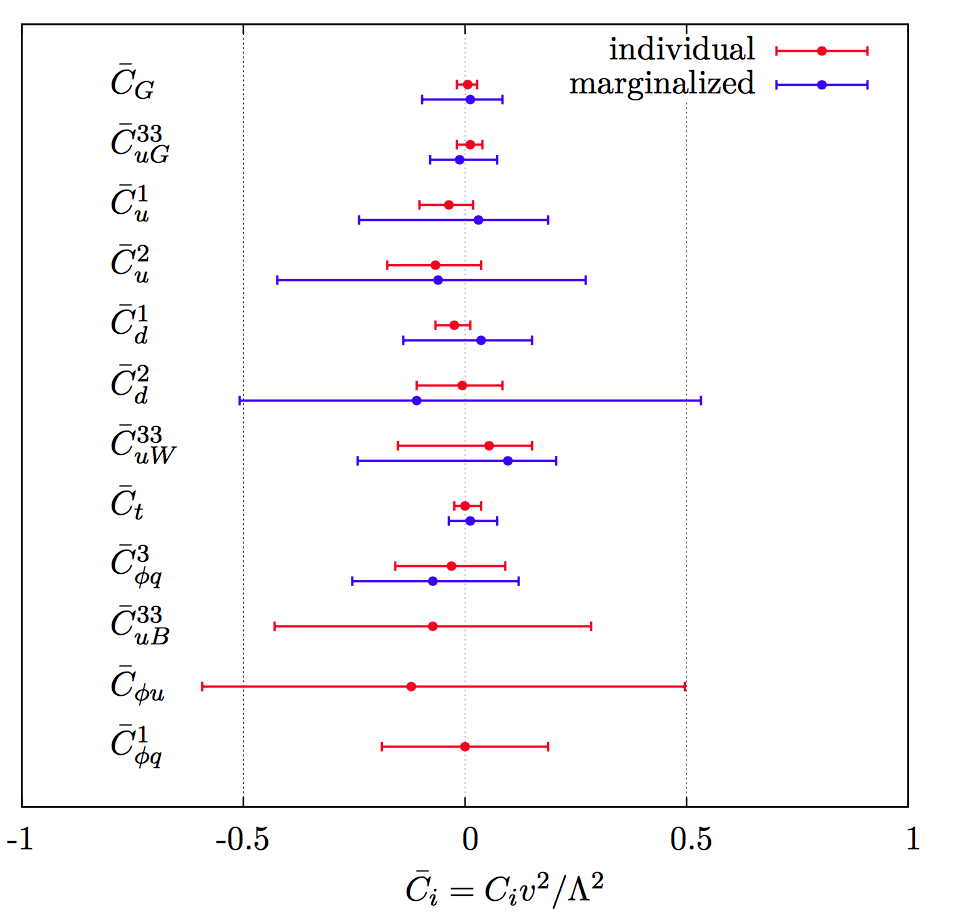
\includegraphics[width=1.0\linewidth]{1_Introduction/Figures/anomlouscouplings}
	\caption{Global fit results of top quark effective field theory to experimental data including all constrained operators at dimension six. For the operators, the Warsaw basis of~\cite{Grzadkowski:2010es} is used. The bounds are set on the Wilson coefficients of various operators contributing to top quark production and decay in two cases (red) all other coefficients set to zero, or (blue) all other coefficients are marginalised over. Figure taken from \cite{Buckley:2015lku}. }
	%https://arxiv.org/pdf/1512.03360.pdf conclusion section
	\label{fig:anomlouscouplings}
\end{figure}

%\section{Experimental results on the \SM\ top quark}
%\label{sec:topexp}
%In this section a selection of experimental results of measurements of the \SM\ is presented.  

%The estimations by the CMS and ATLAS collaborations of the CKM matrix element $V_{\Ptop\Pbottom}$ from single top quark measurement are given in \fig{fig:Vtb}. The most precise estimation of $V_{\Ptop\Pbottom}$ originates from a combination of $t$-channel cross section measurements at 7 and 8~\TeV\ by the CMS collaboration resulting in $|f_{\mathrm{L}}V_{\Ptop\Pbottom}| = 0.998 \pm 0.038$ (exp.) $\pm 0.016$ (theo.). Assuming the $f_{\mathrm{L}} = 1$ and $|V_{\Ptop\Pbottom}| < 1$, this result yields a limit of $|V_{\Ptop\Pbottom}| > 0.92$ at 95\% confidence level. The most recent top quark mass measurements are given in \fig{fig:lhctopmasssep2017}. The CMS combined top quark mass measurement is $m_{\Ptop} = 172.44 \pm 0.48$~\GeV\ from 7 and 8~\TeV\ data. 

%\begin{figure}[htbp]
%	\centering
%	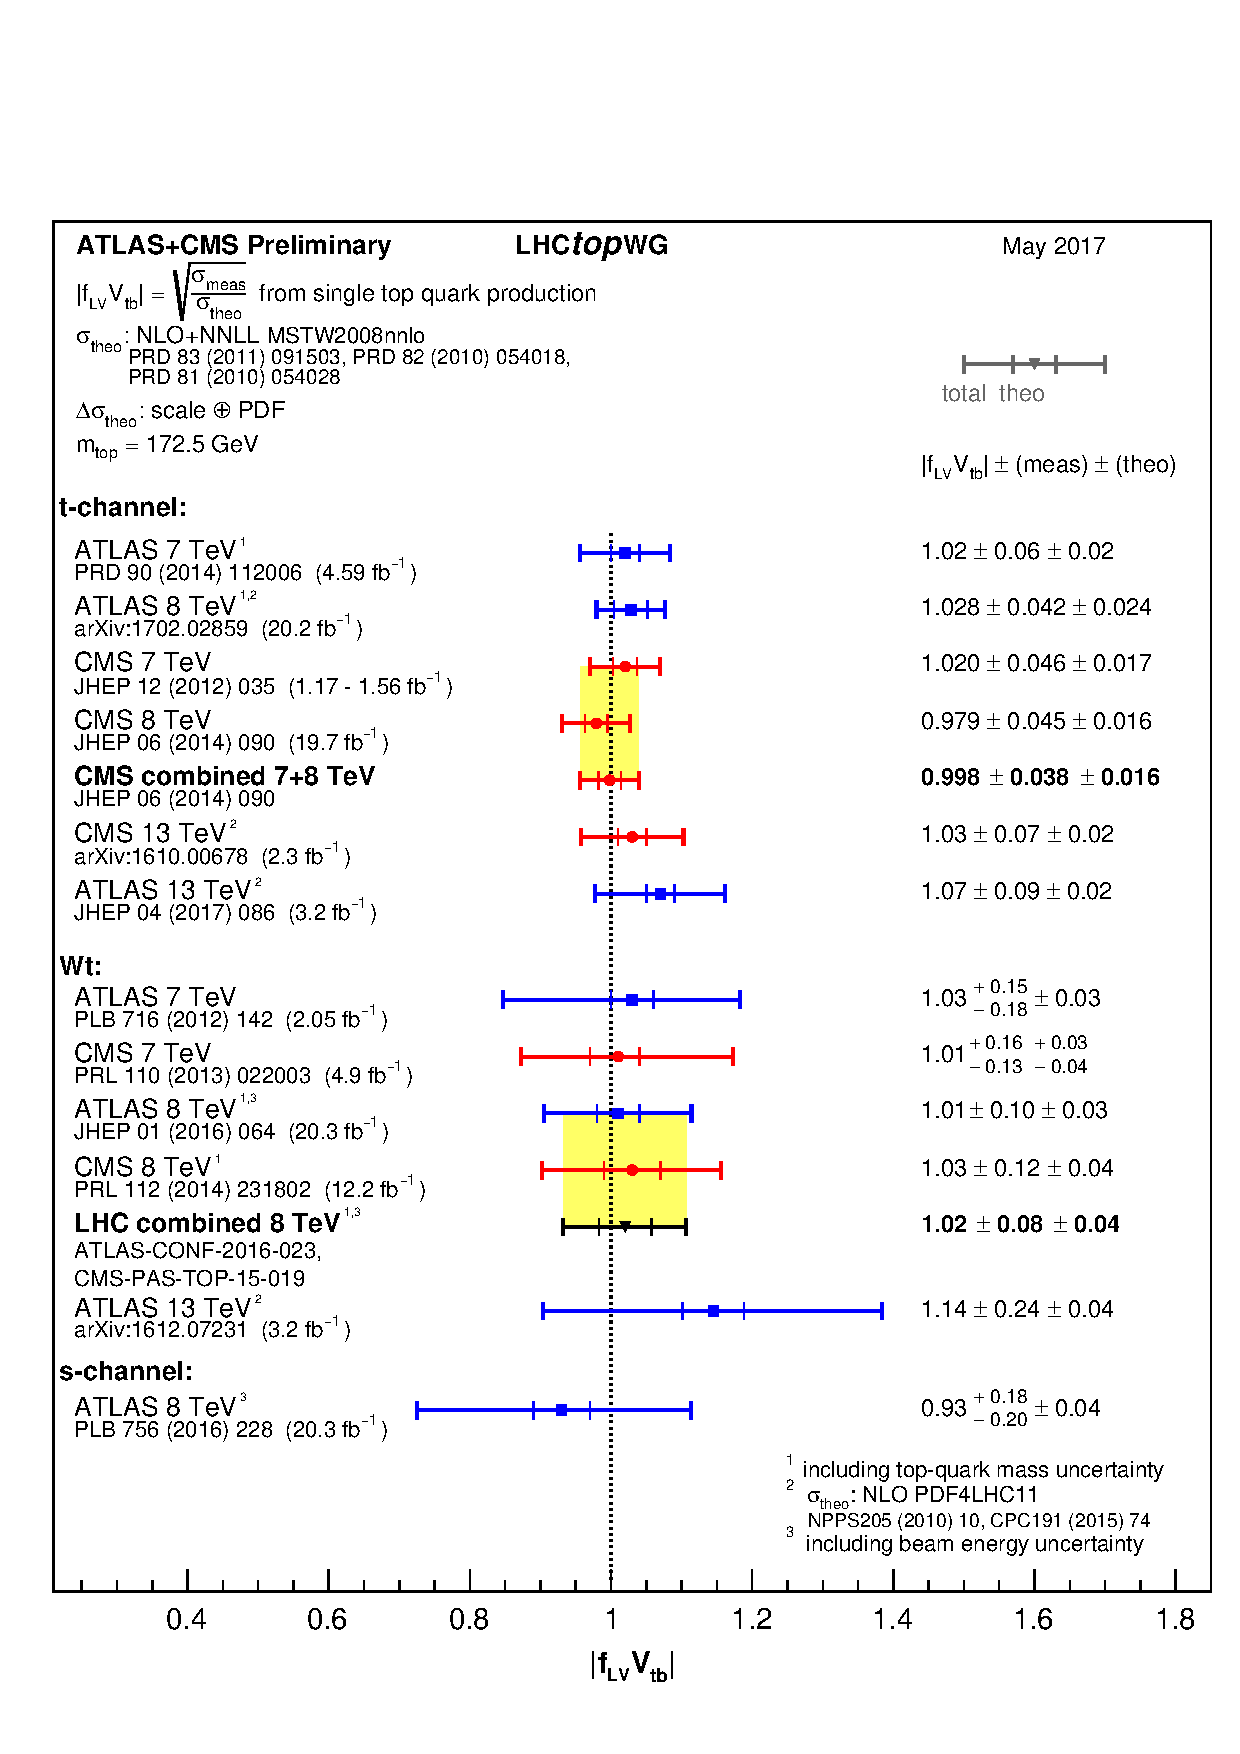
\includegraphics[width=1.\linewidth]{1_Introduction/Figures/singletop_Vtb_may2017}
%	\caption{Estimations of the \SM\ $V_{\Ptop\Pbottom}$ CKM element from single top cross section measurements. Figure taken from \cite{summarytwiki}.}
%	\label{fig:Vtb}
%\end{figure}
%\begin{figure}
%	\centering
%	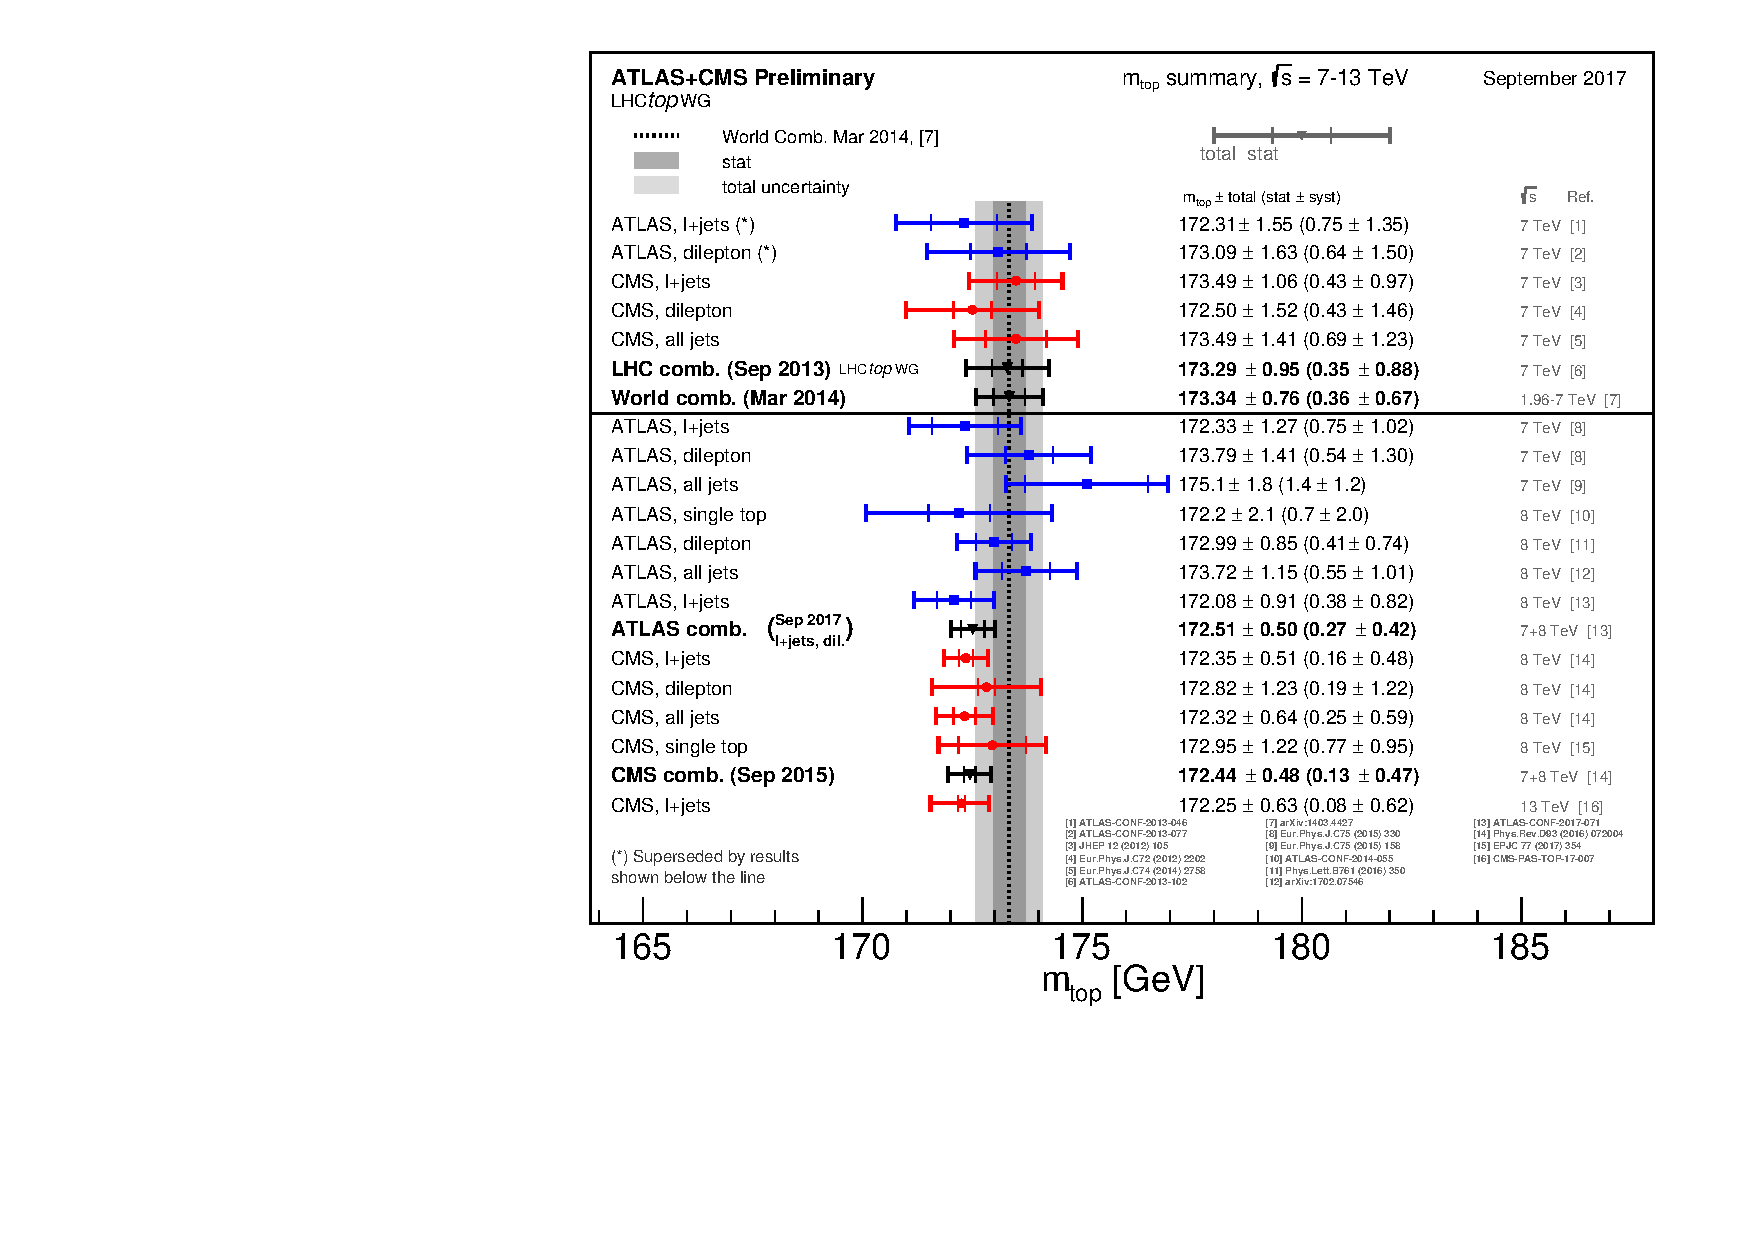
\includegraphics[width=0.7\linewidth]{1_Introduction/Figures/LHC_topmass_sep2017}
%	\caption{Summary of the top mass direct measurements performed by CMS and ATLAS, and compared with the LHC and LHC+Tevatron combinations. The results below the line are produced after the LHC and LHC+Tevatron combinations. Figure taken from \cite{summarytwiki}.}
%	\label{fig:lhctopmasssep2017}
%\end{figure}



\clearpage
\section{Motivation for new physics}
\label{sec:BSM}
Many high energy experiments confirm the success of the \SM. In particular the scalar boson, the cornerstone of the \SM, has consecrated the theory. Unfortunately there are also strong indications that the \SM\ ought to be a lower energy expression of a more global theory. The existence of physics beyond the \SM\ (BSM)~\cite{BSMWiley} is strongly motivated. These motivations are based on direct evidence from observation such as the existence of neutrino masses, the existence of dark matter and dark energy, or the matter-antimatter asymmetry, and also from theoretical problems such as the hierarchy problem, the coupling unification or the large numbers of free parameters in the \SM. 


In the \SM, the neutrinos are assumed to be massless, while experiments with solar, atmospheric, reactor and accelerator neutrinos have established that neutrinos can oscillate and change flavour during flight~\cite{Fukuda:1998mi,PhysRevLett.108.131801}. These oscillations are only possible when neutrinos have masses. The flavour neutrinos (\Pnue, \Pnum, \Pnut) are then linear expressions of the fields of at least three mass eigenstate neutrinos \Pnu$_1$, \Pnu$_2$, and \Pnu$_3$. 

The ordinary or baryonic matter described by the \SM\ describes only 5\% of the mass (energy) content of the universe. Astrophysical evidence indicated that dark matter is contributing to approximately 27\% and dark energy to 68\% of the content of the universe. From the measurements of the temperature and polarizations anisotropies of the cosmic microwave background by the Planck experiment~\cite{Ade:2015xua}, the density of cold non baryonic matter is determined. Cold dark matter is assumed to be only sensitive to the weak and gravitational force, leading to only one possible \SM\ candidate: the neutrino. However, these are too light to account for the vast amount of dark matter and other models are needed. Dark energy is assumed to be responsible for the acceleration in the expansion of the universe~\cite{Peebles:2002gy}. 
%https://en.wikipedia.org/wiki/Accelerating_expansion_of_the_universe#Evidence_for_acceleration

At the Big Bang, matter and antimatter are assumed to be produced in equal quantities. However, it  is clear that we are solely surrounded by matter. In 1967, Sakharov identified three mechanisms that are necessary to obtain a global matter antimatter asymmetry~\cite{Sakharov}. These mechanisms are those of baryon and lepton number violation, that at a given moment in time there was a thermal imbalance for the interactions in the universe, and there is charge C and charge parity CP violation\footnote{The rate of a process $i\rightarrow f$ can be different from the CP-conjugate process: $\tilde i \rightarrow \tilde f$. The \SM\ includes sources of CP-violation through the residual phase of the CKM matrix. However, these could not account for the magnitude of the asymmetry observed.}.
% infor CP viol http://pdg.lbl.gov/2017/reviews/rpp2016-rev-cp-violation.pdf
% CP violation can occur in a filed theory when the lagrangian density involves more complex parameters than what can be removed by field redefinitions

The large number of free parameters in the \SM\ comes from the nine fermion masses, three CKM mixing angles and one CP violating phase, one EM coupling constant $g'$, one weak coupling constant $g$, one strong coupling constant $g_{\mathrm{s}}$, one QCD vacuum angle, one vacuum expectation value, and one mass of the scalar boson. This large number of free parameters leads to the expectation of a more elegant and profound theory beyond the \SM. 

The hierarchy problem~\cite{Burdman:2007ck} is related to the huge difference in energy between the weak scale and the Planck scale. The vev of the Brout-Englert-Higgs field determines the weak scale that is approximately 246~\GeV.  The radiative corrections to the scalar boson squared mass $m_{\PH}^2$, coming from its self couplings and couplings to fermions and gauge bosons, are quadratically proportional to the ultraviolet momentum cut-off $\Lambda_{\mathrm{UV}}$. This cut-off is at least equal to the energy to which the \SM\ is valid without the need of new physics. For the \SM\ to be valid up to the Planck mass, the correction to $m_{\PH}^2$ becomes thirty orders of magnitude larger than $m_{\PH}^2$. This implies that an extraordinary cancellation of terms should happen. This is also known as the naturalness problem of the \PH boson mass. 

The correction to the squared mass of the scalar boson coming from a fermion f, coupling to the scalar field $\phi$ with a coupling $\lambda_{\mathrm{f}}$ is given by
\begin{equation}
\Delta m_{\PH}^2 = -\frac{\left|\lambda_{\mathrm{f}}\right|^2}{8\pi^2}\Lambda_{\mathrm{UV}}^2, 
\end{equation}
while the correction to the mass from a scalar particle S with a mass $m_{\mathrm{S}}$, coupling to the scalar field with a Lagrangian term $-\lambda_{\mathrm{S}}|\phi|^2|\mathrm{S}|^2$ is 
\begin{equation}
\Delta m_{\PH}^2 = \frac{\left|\lambda_{\mathrm{S}}\right|^2}{16\pi^2}\left(\Lambda_{\mathrm{UV}}^2 - 2 m_{\mathrm{S}}^2\; \mathrm{ln}\left(\frac{\Lambda_{\mathrm{UV}}}{m_{\mathrm{S}}}\right) + ...\right). 
\end{equation}
As one can see the correction term to $m_{\PH}^2$ is much larger than $m_{\PH}^2$ itself. By introducing BSM physics models that introduce new scalar particles at the~\TeV\ scale that couple to the scalar boson one can cancel the $\Lambda_{\mathrm{UV}}^2$ divergence and avoid this fine-tuning. 

%https://en.wikipedia.org/wiki/Hierarchy_problem
%https://www.quantumdiaries.org/2012/07/01/the-hierarchy-problem-why-the-higgs-has-a-snowballs-chance-in-hell/
%Also the large mass differences between the fermions related to the Yukawa couplings can go up to six order of magnitude in the case of the electron and the top quark and constitute the fermion mass hierarchy problem. 


The choice of the \SSU\ symmetry group itself  as well as the separate treatment of the three forces included in the \SM\ raises concern. The intensity of the forces show a large disparity around the electroweak scale, but have comparable strengths at higher energies. The electromagnetic and weak forces are unified in a electroweak interaction, but the strong coupling constant does not encounter the other coupling constants at high energies. In order to reach a grand unification, the running of couplings can be modified by the addition of new particles in \BSM\ models. 


\section{An effective approach beyond the \SM: FCNC involving a top quark}
\label{sec:EFT}
% belagrijk om te lezen: https://indico.in2p3.fr/event/11080/contributions/4154/attachments/3112/3770/recap.pdf
%https://mail.google.com/mail/u/0/#search/zeta/1572dd027705dda8
The closeness of the top quark mass to the electroweak scale led physicists to believe that the top quark is a sensitive probe for new physics.  Studying its properties is therefore an important topic of the experimental program at the LHC. Several extensions of the \SM\ enhance the top quark FCNC branching fractions and can be probed at the LHC~\cite{AguilarSaavedra:2004wm}, for which some of them are shown in \tab{tab:FCNCBRnp}. Previous searches have been performed at the Tevatron by the CDF~\cite{PhysRevLett.101.192002} and D0~\cite{Abazov:2010qk} collaborations, 
and at the LHC by the ATLAS~\cite{Aad:2015uza,Aad:2015gea,Aad:2015pja,Aaboud:2017mfd,ATLAS-CONF-2017-070} and CMS~\cite{Sirunyan:2017kkr,Chatrchyan:2013nwa,Khachatryan:2015att,Sirunyan:2017kkr,Khachatryan:2016atv,CMS-PAS-TOP-17-003}  collaborations.
\begin{table}[htbp]
	\centering
	\caption{The predicted branching fractions \BR\ for FCNC interactions involving the top quark in some  \BSM\ models~\cite{AguilarSaavedra:2004wm}: quark singlet (QS), generic two Higgs doublet model (2HDM) and the minimal supersymmetric extensions to the \SM\ (MSSM).}
	\begin{tabular}{lccc}
		\toprule
		Process	& QS & 2HDM & MSSM\\ 
		\midrule
		$ \Ptop \rightarrow \Pup \PZ $     & $\leq 1.1  \times 10^{-4}$&$-$&$\leq 2  \times 10^{-6}$\\
		$ \Ptop \rightarrow \Pup \Pphoton $& $\leq 7.5  \times 10^{-9}$&$-$&$\leq 2  \times 10^{-6}$\\
		$ \Ptop \rightarrow \Pup \Pgluon $ & $\leq 1.5  \times 10^{-7}$&$-$&$\leq 8  \times 10^{-5}$\\
		$ \Ptop \rightarrow \Pup \PHiggs $ & $\leq 4.1  \times 10^{-5}$&$\leq 5.5\;10^{-6}$&$\leq 10^{-5}$ \B    \\
		\hdashline
		$ \Ptop \rightarrow \Pcharm \PZ $      & $\leq 1.1  \times 10^{-4}$& $\leq 10^{-7}$& $\leq 2  \times 10^{-6}$ \T\\
		$ \Ptop \rightarrow \Pcharm \Pphoton $ & $\leq 7.5  \times 10^{-9}$& $\leq 10^{-6}$ &$\leq 2  \times 10^{-6}$\\
		$ \Ptop \rightarrow \Pcharm \Pgluon $  & $\leq 1.5  \times 10^{-7}$&  $\leq 10^{-4}$&$\leq 8  \times 10^{-5}$\\
		$ \Ptop \rightarrow \Pcharm \PHiggs $  & $\leq 4.1  \times 10^{-5}$& $\leq 10^{-3}$&$\leq 10^{-5}$\\
		\bottomrule
	\end{tabular} 
	\label{tab:FCNCBRnp}
\end{table}

The impact of \BSM\ models can be written in a model independent way by means of an effective field theory valid up to an energy scale $\Lambda$.  The leading effects are parametrized by a set of  fully gauge symmetric operators that are added to the \SM\ Lagrangian and can be reduced to a minimal set of operators as seen in \eq{eq:eft}. For simplicity, the assumption is made that new physics effects are exclusively described by dimension-6 operators, thus neglecting neutrino physics. In the fully gauge symmetric case, the EFT Lagrangian is then given by 
\begin{linenomath}
	\begin{equation}
	\Lagr_{\mathrm{SM+EFT}} = \LSM + \sum \limits_{\mathrm{i}} \frac{\bar{c}_{\mathrm{i}}}{\Lambda^2}O_{\mathrm{i}} + \order \left(\frac{1}{\Lambda^3} \right),
	\label{eq:EFTlagrangianf}
	\end{equation}
\end{linenomath}
where the Wilson coefficients $\bar{c}_{\mathrm{i}}$ depend on the considered theory and on the way that new physics couples to the \SM\ particles. Taking into account that $\Lambda$ is large, contributions suppressed by powers of $\Lambda$ greater than two are neglected. Additionally, all four fermion operators are omitted for the rest of this thesis. The Warsaw basis is adopted for the independent effective operators~\cite{Grzadkowski:2010es}, parametrising the new physics effects relevant for the flavour changing neutral current interactions of the top quark as, 
\begin{equation}
	\begin{aligned}
	\Lagr^{\Ptop}_{\mathrm{EFT}}  &= 
	\frac{\bar{c}_{ uG}}{\Lambda^2}
	\Phi^{\dagger} \!\cdot\!
	\left[ \bar{Q}_{\mathrm{L}} \sigma^{\mu\nu} \mathcal{T}_a u_{\mathrm{R}}\right] G^a_{\mu\nu} +
	\frac{\bar{c}_{ uB}}{\Lambda^2}
	\Phi^{\dagger} \!\cdot\!
	\left[ \bar{Q}_{\mathrm{L}} \sigma^{\mu\nu} u_{\mathrm{R}}\right] B_{\mu\nu} +
	\frac{2 \bar{c}_{ uW}}{\Lambda^2}
	\Phi^{\dagger} {T}_{\mathrm{i}} \!\cdot\!
	\left[ \bar{Q}_{\mathrm{L}} \sigma^{\mu\nu} u_{\mathrm{R}}\right] W^{\mathrm{i}}_{\mu\nu} \\
    &  +\ i \frac{\bar{c}_{ hu}}{\Lambda^2}
	\left[ \Phi^{\dagger} \overleftrightarrow{D}_\mu \Phi \right]
	\left[ \bar{u}_{\mathrm{R}} \gamma^\mu u_{\mathrm{R}}\right] 
	+ i \frac{\bar{c}_{ hq}^{(1)}}{\Lambda^2}
	\left[ \Phi^{\dagger} \overleftrightarrow{D}_\mu \Phi \right] 
	\left[ \bar{Q}_{\mathrm{L}} \gamma^{\mu} Q_{\mathrm{L}} \right] \\
	&\ +  \ i \frac{4 \bar{c}_{h\Pquark}^{(3)}}{\Lambda^2}
	\left[ \Phi^{\dagger} {T}_{i} \overleftrightarrow{D}_\mu \Phi \right]
	\left[ \bar{Q}_{\mathrm{L}} \gamma^\mu { T}^{\mathrm{i}} Q_{\mathrm{L}}\right]
	+  \frac{\bar{c}_{uh}}{\Lambda^2} \Phi^{\dagger}\Phi\ 
	\Phi^{\dagger} \cdot \left[ \bar{Q}_{\mathrm{L}} u_{\mathrm{R}}\right]
	+ \mathrm{ h.c.} \ ,
	\end{aligned}
	\label{eq:Wil}
\end{equation}
with all flavour indices implied. The left handed \Stwo\ doublet of the quark fields is denoted by $Q_{\mathrm{L}}$, the up-type right handed fields by $u_{\mathrm{R}}$,  the \Stwo\ doublet of the Higgs field by $\Phi$, the field strength tensors as 
\begin{equation}
	\begin{aligned}
	B_{\mu\nu} &= \partial_{\mu} B_{\nu} - \partial_{\nu} B_{\mu}, \\
	W_{\mu\nu}^{\mathrm{k}} &= \partial_{\mu} W_{\nu}^{\mathrm{k}} - \partial_{\nu} W_{\mu}^{\mathrm{k}}-g\epsilon_{\mathrm{ij}}^{\mathrm{k}}W_{\mu}^{\mathrm{i}}W_{\nu}^{\mathrm{j}},\\
    	\Gtensor^{\mathrm{a}} &= \partial_{\mu} \mathrm{G}_{\nu}^{\mathrm{a}} -  \partial_{\nu}  \mathrm{G}_{\mu}^{\mathrm{a}} + g_{\mathrm{s}} f^{\mathrm{a}}_{\mathrm{bc}}   \mathrm{G}_{\mu}^{\mathrm{b}} \mathrm{G}_{\nu}^{\mathrm{c}} , 
	\end{aligned}
\end{equation}
denoting the structure constant of the \Sthree\ group  as $f^{\mathrm{a}}_{\mathrm{bc}}$ and the structure constant of the \Stwo\ group as $\epsilon_{\mathrm{ij}}^{\mathrm{k}}$. The gauge covariant derivatives are  defined as 
\begin{equation}
D_{\mu} \Phi   = \partial_{\mu} \Phi - \frac{1}{2}ig'B_{\mu}\Phi - igT_{\mathrm{k}}W_{\mu}^{\mathrm{k}}\Phi
\end{equation}
with the conventions of \Sec{sec:SMlagr}. The representation matrices $T$ of \Stwo\ are defined in \eq{eq:Stwee} and are half the Pauli matrices, while the representation matrices $\mathcal{T}$ of \Sthree\ are the Gell-Mann matrices~\cite{Peskin:257493}. The hermitian derivative operator is defined as 
\begin{equation}
	\Phi^{\dagger}\overleftrightarrow{D}\Phi = \Phi^{\dagger}D^{\mu}\Phi - D_{\mu}\Phi^{\dagger}\Phi.
\end{equation}

 After electroweak symmetry breaking,  the operators induce~\cite{AguilarSaavedra:2004wm,Beneke:2000hk} both corrections to the \SM\ couplings and new interactions at tree level such as FCNC interactions. The Lagrangian of \eq{eq:Wil} can then equivalently be written as  
 \begin{equation}
\begin{aligned}
\Lagr^{\Ptop}_{\mathrm{EFT}} =\frac{\sqrt{2}}{2}\sum\limits_{\Pquark = \Pup,\Pcharm} &\left[g'
\frac{\kfqt}{\Lambda} \photontensor \APtop \sigma^{\mu\nu}\left(f^{\mathrm{L}}_{\Pphoton\Pquark} P_{\mathrm{L}} + f^{\mathrm{R}}_{\Pphoton\Pquark} P_{\mathrm{R}}\right) \Pquark \right. \\
&+ \frac{g}{2\cW} \frac{\kZqt}{\Lambda} \Ztensor \APtop \sigma^{\mu\nu}\left(f^{\mathrm{L}}_{\PZ\Pquark} P_{\mathrm{L}} + f^{\mathrm{R}}_{\PZ\Pquark} P_{\mathrm{R}}\right) \Pquark \\
&+\frac{\sqrt{2}g}{4\cW} \zZqt \APtop \gamma^{\mu} \left(\tilde{f}^{\mathrm{L}}_{\Pquark} P_{\mathrm{L}} + \tilde{f}^{\mathrm{R}}_{\Pquark} P_{\mathrm{R}}\right) \Pquark \PZ_{\mu} \\
&+ g_{\mathrm{s}} \frac{\kgqt}{\Lambda}  \APtop \sigma^{\mu\nu} \mathcal{T}_{\mathrm{a}} \left(f^{\mathrm{L}}_{\Pgluon\Pquark} P_{\mathrm{L}} + f^{\mathrm{R}}_{\Pgluon\Pquark} P_{\mathrm{R}}\right) \Pquark \Gtensor^{\mathrm{a}}\\
&+ \left. \eta_{\PHiggs\Pquark\Ptop} \APtop\left(\hat{f}^{\mathrm{L}}_{\Pquark} P_{\mathrm{L}} + \hat{f}^{\mathrm{R}}_{\Pquark} P_{\mathrm{R}}\right) \Pquark \PHiggs + \mathrm{h.c.}\right],
\label{eq:EFTlag}
\end{aligned}
\end{equation}
which gives the FCNC interactions of the top quark that are not present in the \SM. The value of the \FCNC\ couplings at scale $\Lambda$ are represented by \kZqt, \kgqt, \kfqt, \zZqt, and ${ \eta_{{\PHiggs\Pquark \Ptop}}}$. These are assumed to be real and positive, with the unit of $\GeV^{-1}$ for $\kxqt$ and no unit for $\zeta_{xqt}$ and $\eta_{\mathrm{xqt}}$. In the equation, $\sigma^{{\mu \nu}}$ equals to $\frac{i}{2}\left[\gamma^{{\mu}},\gamma^{\nu}\right]$,  and the left- and right-handed chirality projector operators are denoted by $P_{\mathrm{L}}$ and $P_{\mathrm{R}}$. The electromagnetic coupling constant is denoted by $g'$, the strong interaction coupling is denoted as $g_{\mathrm{s}}$, while the electroweak interaction is parametrised by the coupling constant $g$ and the electroweak mixing angle $\theta_{\mathrm{W}}$.  The complex chiral parameters are normalized according to
$ |f_{\mathrm{xq}}^{\mathrm{L}}|^2 + |f_{\mathrm{xq}}^{\mathrm{R}}|^2 = 1 $, $|\tilde{f}_{\mathrm{q}}^{\mathrm{L}}|^2 + |\tilde{f}_{\mathrm{q}}^{\mathrm{R}}|^2 = 1$, and $|\hat{f}_{\mathrm{q}}^{\mathrm{L}}|^2 + |\hat{f}_{\mathrm{q}}^{\mathrm{R}}|^2 = 1$. In the expression for $\Lagr^{\Ptop}_{\mathrm{EFT}}$, the unitary gauge is adopted and the scalar field is expanded around its vacuum expectation value $v$ with \PHiggs\ being the \SM\ Higgs boson. The field strength tensors of the photon \photonfield, the gluon field \Gfields, and the \PZ\ boson \Zfield\ are defined as
\begin{equation}
\begin{aligned}
	\photontensor &= \partial_{\mu} \mathrm{A}_{\nu} -  \partial_{\nu} \mathrm{A}_{\mu}, \\
	  \PZ_{\mu\nu} &= \partial_{\mu} \mathrm{Z}_{\nu} -  \partial_{\nu} \mathrm{Z}_{\mu},\: \mathrm{ and } \\
	\Gtensor^{\mathrm{a}} &= \partial_{\mu} \mathrm{G}_{\nu}^{\mathrm{a}} -  \partial_{\nu}  \mathrm{G}_{\mu}^{\mathrm{a}} + g_{\mathrm{s}} f^{\mathrm{a}}_{\mathrm{bc}}   \mathrm{G}_{\mu}^{\mathrm{b}} \mathrm{G}_{\nu}^{\mathrm{c}}.
	\end{aligned}
\end{equation}
 
 
 \newpage
 The relations between the Wilson coefficients in \eqref{eq:Wil} and the coupling strengths of the interactions in \eq{eq:EFTlag} can be derived. The 14 effective operators are mapped onto 10 free parameters providing a more minimal parametrisation of the anomalous interactions of the top quark:
% \renewcommand{\arraystretch}{1.2}
\begin{equation}
\begin{array}{l l}
 	\kgqt f^{\mathrm{L}}_{\Pgluon\Pquark} = \frac{v}{g_{\mathrm{s}} \Lambda}
 	\left[\bar{c}_{ uG}\right]_{i3}^\ast\ ,
 	\ \   &
 	\kgqt f^{\mathrm{R}}_{\Pgluon\Pquark} \!=\! \frac{v}{g_{\mathrm{s}} \Lambda}
 	\left[\bar{c}_{ uG}\right]_{3i}\ , \\
 	%
 	\kfqt f^{\mathrm{L}}_{\Pphoton\Pquark} = \frac{v}{g' \Lambda}
 	\left[\cw \bar{c}_{ uB} - \sw \bar{c}_{ uW}\right]_{i3}^\ast\ ,
 	\ \   &
 	\kfqt f^{\mathrm{R}}_{\Pphoton\Pquark} \!=\! \frac{v}{g' \Lambda}
 	\left[\sw \bar{c}_{ uB} - \cw \bar{c}_{ uW}\right]_{3i} \ ,\\
 	%
 	\kZqt f^{\mathrm{L}}_{\PZ\Pquark} = -\frac{2 \cw v}{g \Lambda}
 	\left[\sw \bar{c}_{ uB} + \cw \bar{c}_{ uW}\right]_{i3}^\ast\ ,
 	\ \   &
 	\kZqt f^{\mathrm{R}}_{\PZ\Pquark} \!=\! -\frac{2 \cw v}{g \Lambda}
 	\left[\cw \bar{c}_{ uB} \!+\! \sw \bar{c}_{ uW}\right]_{3i} \ ,\\
 	%
 	\zZqt \tilde f^{\mathrm{L}}_{\PZ\Pquark} = - \frac{2 v^2}{\Lambda^2}
 	\left[\big(\bar{c}_{ hq}^{(1)}\!-\!\bar{c}_{ hq}^{(3)}\big)_{i3} \!+\!
 	\big(\bar{c}_{ hq}^{(1)}\!-\!\bar{c}_{ hq}^{(3)}\big)_{3i}^\ast\right]\ ,
 	\ &
 	\zZqt \tilde f^{\mathrm{R}}_{\PZ\Pquark} \!=\! - \frac{2 v^2}{\Lambda^2}
 	\left[(\bar{c}_{ hu})_{i3} + (\bar{c}_{ hu})_{3i}^\ast\right] \ ,\\
 	%
 	\eta_{\Ptop\PH\Pquark} \hat f^{\mathrm{L}}_{\PH\Pquark} = \frac{3 v^2}{2 \Lambda^2}
 	\left[\bar{c}_{ uh}\right]_{3i}^\ast\ ,
 	\ &
 	\eta_{\Ptop\PH\Pquark} \hat f^{\mathrm{R}}_{\PH\Pquark} \!=\! \frac{3 v^2}{2 \Lambda^2}
 	\left[\bar{c}_{ uh}\right]_{i3} .\\
 \end{array}
\end{equation}

 
\begin{comment}
\begin{linenomath}
	\begin{equation}
	\begin{aligned}
	\Lagr_{\mathrm{SM+EFT}} &= \sum \limits_{{\Pquark=\Pup,\Pcharm,\Ptop}} \left[ 
	\frac{\sqrt 2}{2} {g_{\mathrm{s}}} { \frac{\kgqt}{\Lambda}} \APtop \sigma^{\mu \nu} \left( {f_{{\Pgluon\Pquark}}^{\mathrm{L}}} P_{\mathrm{L}} + {f_{{\Pgluon\Pquark}}^{\mathrm{R}}}P_{\mathrm{R}}\right) \Pquark \Gtensor^{\mathrm{a}} 
	+ \frac{\sqrt 2}{2} e { \frac{\kfqt}{\Lambda}} \APtop \sigma^{\mu \nu} \left( {f_{\Pphoton \Pquark}^{\mathrm{L}}} P_{\mathrm{L}} + {f_{\Pphoton \Pquark}^{\mathrm{R}}}P_{\mathrm{R}}\right) \Pquark \photontensor  \right.\\
	&+ \frac{1}{\sqrt 2}  { \eta_{{\PHiggs\Pquark \Ptop}}} \APtop  \left( {f_{\PHiggs \Pquark }^{\mathrm{L}}} P_{\mathrm{L}} + {f_{{\PHiggs \Pquark }}}^{\mathrm{R}}P_{\mathrm{R}}\right) \Pquark \PHiggs 
	+ \frac{\sqrt 2}{4} {\frac{g}{\cW}} { \frac{\kZqt}{\Lambda}} \APtop \sigma^{\mu \nu} \left( {f_{{\PZ\Pquark}}^{\mathrm{L}}} P_{\mathrm{L}} + {f_{{\PZ\Pquark}}^{\mathrm{R}}} P_{\mathrm{R}}\right) \Pquark \Ztensor \\
	&\left. + \frac{1}{4} {\frac{g}{\cW}} { \zZqt} \APtop \gamma^{\mu} \left( {\tilde{f}_{{\PZ\Pquark}}^{\mathrm{L}}} P_{\mathrm{L}} + {\tilde{f}_{{\PZ\Pquark}}^{\mathrm{R}}}P_{\mathrm{R}}\right) \Pquark \PZ_{\mu} \right] + \mathrm{h.c.} \\
	&+ \sum \limits_{\Pquark=\Pdown,\Pstrange,\Pbottom} \left[ \frac{1}{2} {g} { \frac{\kappa_{\Ptop\PW\Pquark}}{\Lambda}} \APtop \sigma^{\mu \nu} \left( {f_{\PW \Pquark}^{\mathrm{L}}} P_{\mathrm{L}} + {f_{\PW \Pquark}^{\mathrm{R}}}P_{\mathrm{R}}\right) \Pquark \PW^+_{\mu \nu} + \frac{\sqrt 2}{4} {g} { \zWqt} \APtop \gamma^{{\mu} } \left( {\tilde{f}_{{\PW \Pquark}}^{\mathrm{L}}} P_{\mathrm{L}} + {\tilde{f}_{{\PW \Pquark}}^{\mathrm{R}}}P_{\mathrm{R}}\right) \Pquark \PW^+_{{\mu}} \right] \\ 
	&+ \mathrm{h.c.} , 
	\end{aligned}
	\label{eq:EFTlagrangianexpanded}
	\end{equation}
\end{linenomath}
where the value of the \FCNC\ couplings at scale $\Lambda$ are represented by \kZqt,\kgqt,\kfqt,\zZqt, and ${ \eta_{{\PHiggs\Pquark \Ptop}}}$. These are assumed to be real and positive, with the unit of $\GeV^{-1}$ for $\kxqt$ and no unit for $\zeta_{xqt}$ and $\eta_{\mathrm{xqt}}$. In the equation $\sigma^{{\mu \nu}}$ equals to $\frac{i}{2}\left[\gamma^{{\mu}},\gamma^{\nu}\right]$,  and the left- and right-handed chirality projector operators are denoted by $P_{\mathrm{L}}$ and $P_{\mathrm{R}}$. The electromagnetic coupling constant is denoted by $e$, the strong interaction coupling is denoted as $g_{\mathrm{s}}$, while the electroweak interaction is parametrised by the coupling constant $g$ and the electroweak mixing angle $\theta_{\mathrm{W}}$.  The complex chiral parameters and are assumed to be real  and  fulfil the relation 
$ \left(|f_{\mathrm{xq}}^{\mathrm{L}}|^2 + |f_{\mathrm{xq}}^{\mathrm{R}}|^2 \right)= 1 $ and $\left(|\tilde{f}_{\mathrm{xq}}^{\mathrm{L}}|^2 + |\tilde{f}_{\mathrm{xq}}^{\mathrm{R}}|^2 \right)= 1$.
% The limitations of the electro weak broken phase approach are summarised in \cite{Durieux:2014xla}. 

\end{comment}

\section{Experimental constraints on top-FCNC}
\label{sec:ExpConstr}
Experimental particle physicists commonly put limits on the branching fractions which allow an easier interpretation across different EFT models. The branching fraction takes a value between zero and one and is defined as
\begin{equation}
	\BR(\Ptop \rightarrow \Pquark\mathrm{X}) = \frac{\delta^2_{\Ptop \mathrm{X}\Pquark}\Gamma_{\Ptop \rightarrow \Pquark\mathrm{X}}}{\Gamma_{\Ptop}},
	\label{eq:BR}
\end{equation}
 where $\Gamma_{\Ptop \rightarrow \Pquark\mathrm{X}}$ represents the \FCNC\ decay width\footnote{The decay width of a certain process represents the probability per unit time that a particle will decay. The total decay width, defined as the sum of all possible decay widths of a particle, is inversely proportional to its lifetime. } for a coupling strength $\delta^2_{\Ptop \mathrm{X}\Pquark}=1$, and $\Gamma_{\Ptop}$ the full decay width of the top quark. In the \SM, supposing a top quark mass of 172.5~\GeV, the full width becomes $\Gamma_{\Ptop}^{\mathrm{SM}} = 1.32$~\GeV~\cite{Gao:2012ja}. 

% top FCNC vertex in Feynman diagram -> matrix element maal kappa --> cross sectie maal kappa^2 --> cross sectie maal BR (lineair)


Searches for top-FCNC usually adopt a search strategy depending on the experimental set-up and the FCNC interaction of interest,  looking either for \FCNC\ interactions in the production of a single top quark or in its decay for top quark pair interactions. In \fig{fig:Feynman}, these two cases are shown for the \tZq\ vertex.  \\
\begin{figure}[hbtp]
	\centering
	\subbottom[]{
			\begin{fmffile}{singletop}
		\begin{fmfgraph*}(160,40) % width - height
\fmfleft{i1,i2} 
\fmfright{o1,o2}
 \fmf{fermion}{i1,v1,v2,o2}
  \fmf{boson}{v2,o1}
   \fmf{gluon}{i2,v1}
   \fmflabel{\Pgluon}{i2}
   \fmflabel{\Pup,\Pcharm}{i1}
   	\fmfv{label= ,decor.shape=circle,decor.filled=shaded,decor,size=0.5thick, label.angle=-90}{v2}
  % \fmflabel{\Pup,\Pcharm}{i1}
   \fmflabel{\PZ}{o1}
   \fmflabel{\Ptop}{o2}
    \fmf{fermion,label=\Pup,,\Pcharm,label.dist=10}{v1,v2}
      \end{fmfgraph*}
\end{fmffile}
}
\hspace*{1cm}
\subbottom[]{
	\begin{fmffile}{toppair}
	\begin{fmfgraph*}(160,40) % width - height
		\fmfleft{i1,i2} 
		\fmfright{o1,o2,o3,o4}
		\fmflabel{\Pgluon}{i1}
		\fmflabel{\Pgluon}{i2}
		\fmflabel{\APup,\APcharm}{o1}
		\fmflabel{\PZ}{o2}
		\fmflabel{\PWp}{o3}
		\fmflabel{\Pbottom}{o4}
		\fmf{gluon}{i1,v1,i2}
		\fmf{gluon,label=\Pgluon,label.dist=10}{v1,v2}
		\fmf{fermion}{o1,v4,v2,v3,o4}
		\fmffreeze
		\fmf{boson}{v3,o3}
		\fmf{boson}{v4,o2}
		\fmfv{label= ,decor.shape=circle,decor.filled=shaded,decor,size=0.2thick, label.angle=-90}{v4}
		 \fmf{fermion,label=\Ptop,label.dist=5}{v2,v3}
		 \fmf{fermion,label=\APtop,label.dist=-20}{v4,v2}
		\fmflabel{}{v3}
		\fmflabel{}{v2}
		\fmflabel{}{v1}
	\end{fmfgraph*}
\end{fmffile}
}
\caption{Feynman diagrams for the processes with a \tZq\ \FCNC\ interaction, where the FCNC interaction is indicated with the shaded dot. (a) Single top quark production through an \FCNC\ interaction. (b) Top quark pair production with an \FCNC\ induced decay. }
\label{fig:Feynman}
\end{figure}


The observation of top-FCNC interactions has yet to come and experiments have so far only been able to put upper bounds on the branching fractions. An overview of the best current limits is given in \tab{tab:FCNClimits}. In \fig{fig:fcncupperlimits} a comparison is shown between the current best limits set by ATLAS and CMS with respect to several \BSM\ model benchmark predictions. From there one can see that \FCNC\ searches involving a \PZ\ or \PHiggs\ boson are close to excluding or confirming several \BSM\ theories. In \fig{fig:summaryfcnc}, the searches performed by CMS are summarised. For the tZq vertex, the current most stringent limit is set by the ATLAS collaboration at a centre-of-mass energy of 13~\TeV~\cite{ATLAS-CONF-2017-070}. The observed (expected) limits at 95\% CL are $\BR(\Ptop \rightarrow \Pup\PZ) <  1.7 \times 10^{-4}\; (2.4  \times 10^{-4})$ and  $\BR(\Ptop \rightarrow \Pcharm\PZ) < 2.3 \times 10^{-4} \; (3.2 \times 10^{-4})$.  The most stringent limit from the CMS collaboration comes from Ref.~\cite{Sirunyan:2017kkr} where both single top quark and top quark pair processes are studied. The observed (expected) limits at 95\% CL for a centre-of-mass energy of 8~\TeV\ for the FCNC tZq interaction by CMS are $\BR(\Ptop \rightarrow \Pup\PZ) <  2.2 \times 10^{-4}\; (2.7  \times 10^{-4})$ and  $\BR(\Ptop \rightarrow \Pcharm\PZ) < 4.9 \times 10^{-4} \; (12 \times 10^{-4})$.  In \fig{fig:FCNCATLASCMS}, the summary of the 95\% confidence level observed limits on the branching fractions of the top quark decays to a charm or up quark and a neutral boson is given, considering the results from the HERA, the LEP, the Tevatron, and the LHC.
\begin{table}[htbp]
	\centering
	\caption{Overview of the most stringent observed and expected experimental limits on top-FCNC branching fractions \BR\ at 95\% confidence level.}
	\begin{tabular}{llllll}
		\toprule
		Process &Search mode & Observed \BR & Expected \BR & \multicolumn{2}{c}{Experiment} \\ 
		\midrule
%		$\Ptop \rightarrow \Pup\PZ$		     & \tt\ decay  and \st\ production & 2.2 $\times 10^{-4}$& 2.7 $\times 10^{-4}$   & CMS&\cite{Sirunyan:2017kkr}\\
        $\Ptop \rightarrow \Pup\PZ$		     & \tt\ decay   & 1.7 $\times 10^{-4}$& 2.4 $\times 10^{-4}$   & ATLAS&\cite{ATLAS-CONF-2017-070} \\
		$\Ptop \rightarrow \Pup\Pphoton$	 & \st\ production   & 1.3 $\times 10^{-4}$& 1.9 $\times 10^{-4}$& CMS&\cite{Khachatryan:2015att}     \\
		$\Ptop \rightarrow \Pup\Pgluon$		 & \st\ production   & 4.0   $\times 10^{-5}$& 3.5   $\times 10^{-5}$& ATLAS&\cite{Aad:2015gea}   \\
		$\Ptop \rightarrow \Pup\PHiggs$		 & \tt\ decay        & 2.4 $\times 10^{-3}$& 1.7 $\times 10^{-3}$& ATLAS&\cite{Aaboud:2017mfd}   \\
%		$\Ptop \rightarrow \Pcharm\PZ$		 & \tt\ decay  and \st\ production        & 4.9 $\times 10^{-4}$& 12  $\times 10^{-4}$& CMS&\cite{Sirunyan:2017kkr}\\
        $\Ptop \rightarrow \Pcharm\PZ$		 & \tt\ decay        & 2.3 $\times 10^{-4}$& 3.2  $\times 10^{-4}$& ATLAS&\cite{ATLAS-CONF-2017-070}\\
		$\Ptop \rightarrow \Pcharm\Pphoton$  & \st\ production   & 2.0 $\times 10^{-3}$& 1.7 $\times 10^{-3}$& CMS&\cite{Khachatryan:2015att}     \\
		$\Ptop \rightarrow \Pcharm\Pgluon$   & \st\ production   & 2.0   $\times 10^{-4}$& 1.8 $\times 10^{-4}$& ATLAS&\cite{Aad:2015gea}   \\
		$\Ptop \rightarrow \Pcharm\PHiggs$   & \tt\ decay     & 2.2  $\times 10^{-3}$& 1.6 $\times 10^{-3}$& CMS&\cite{Aaboud:2017mfd}     \\
		\bottomrule
	\end{tabular} 
	\label{tab:FCNClimits}
\end{table}

\begin{figure}[htbp]
	\centering
	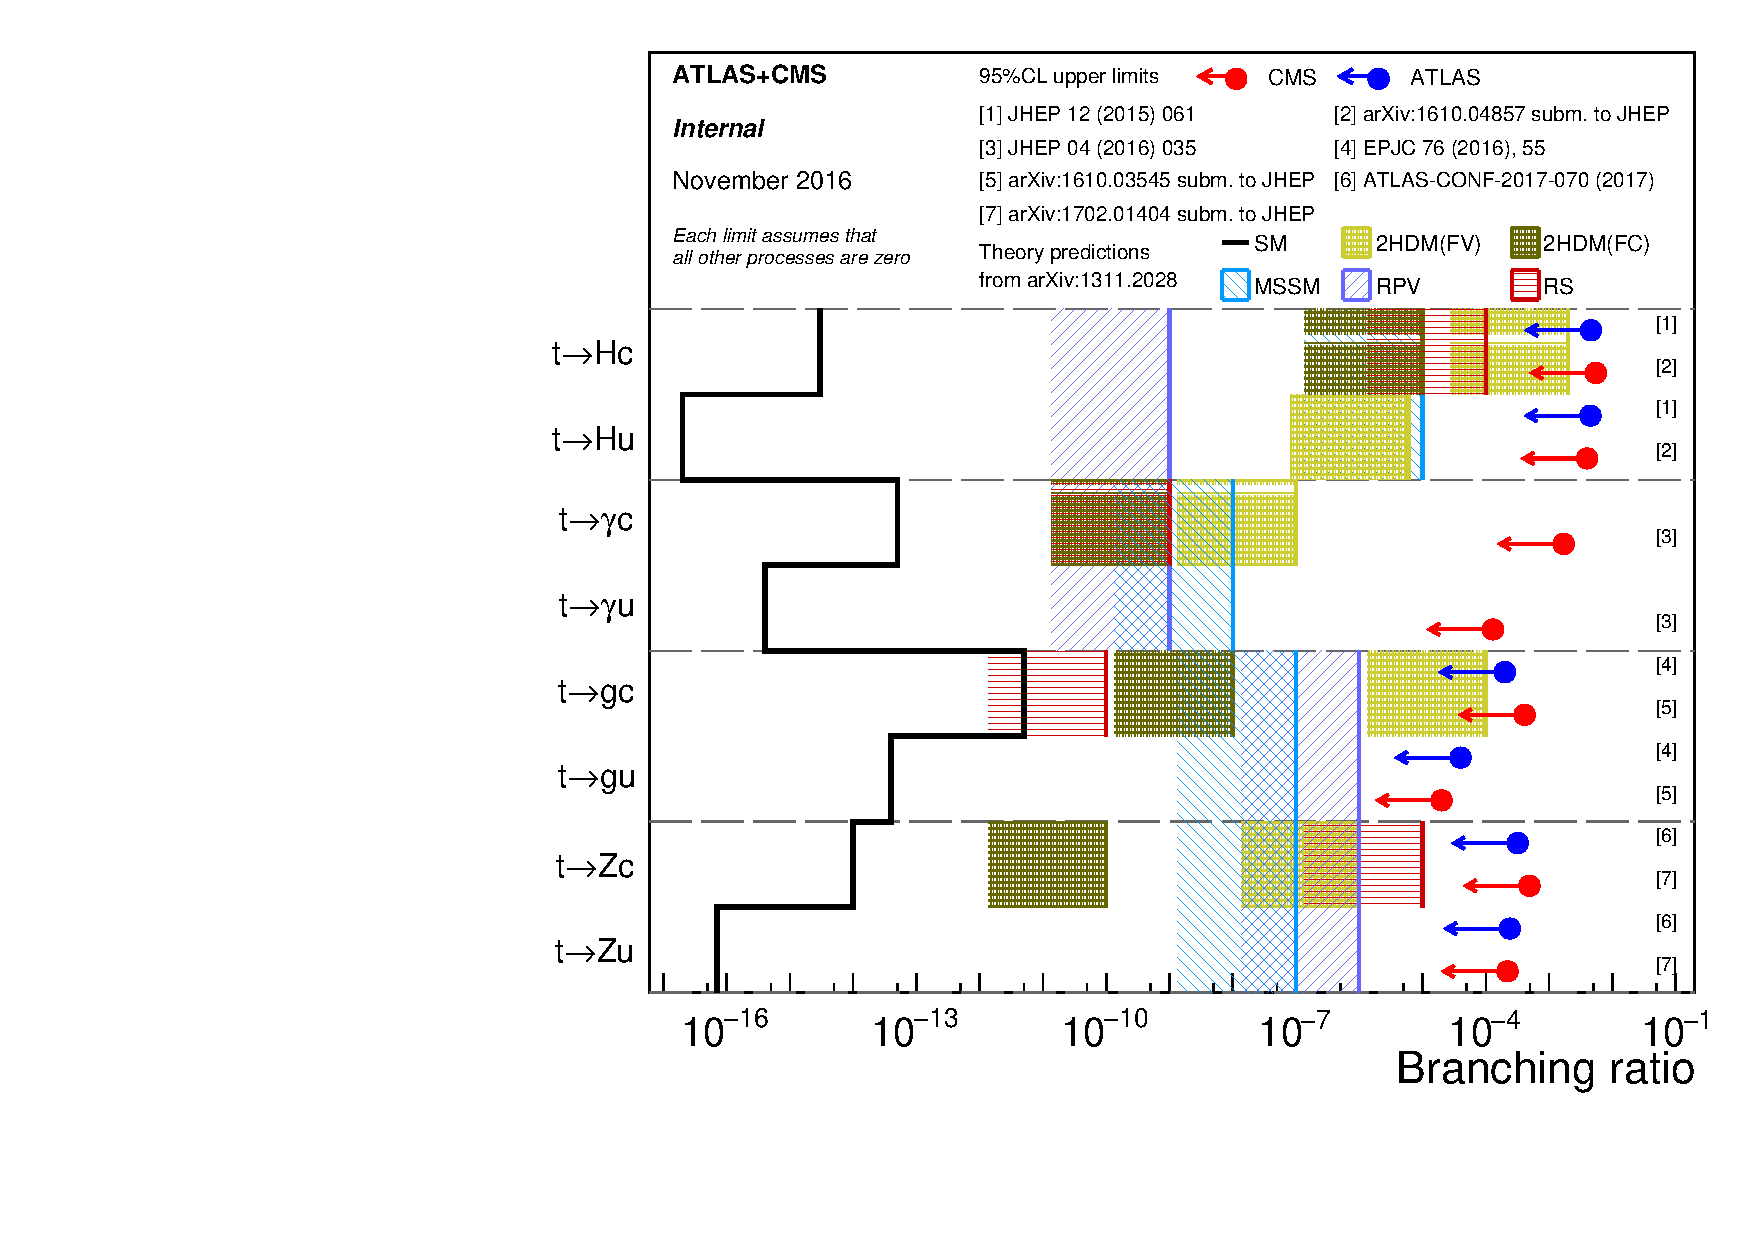
\includegraphics[width=1.\linewidth]{1_Introduction/Figures/fcnc_upperlimitsth.pdf}
	\caption{Current best limits at 95\% confidence level on the branching fractions set by CMS and ATLAS for top-FCNC interactions. Figure adapted from~\cite{summarywiki}. }
	\label{fig:fcncupperlimits}
\end{figure}
\begin{figure}[htbp]
	\centering
	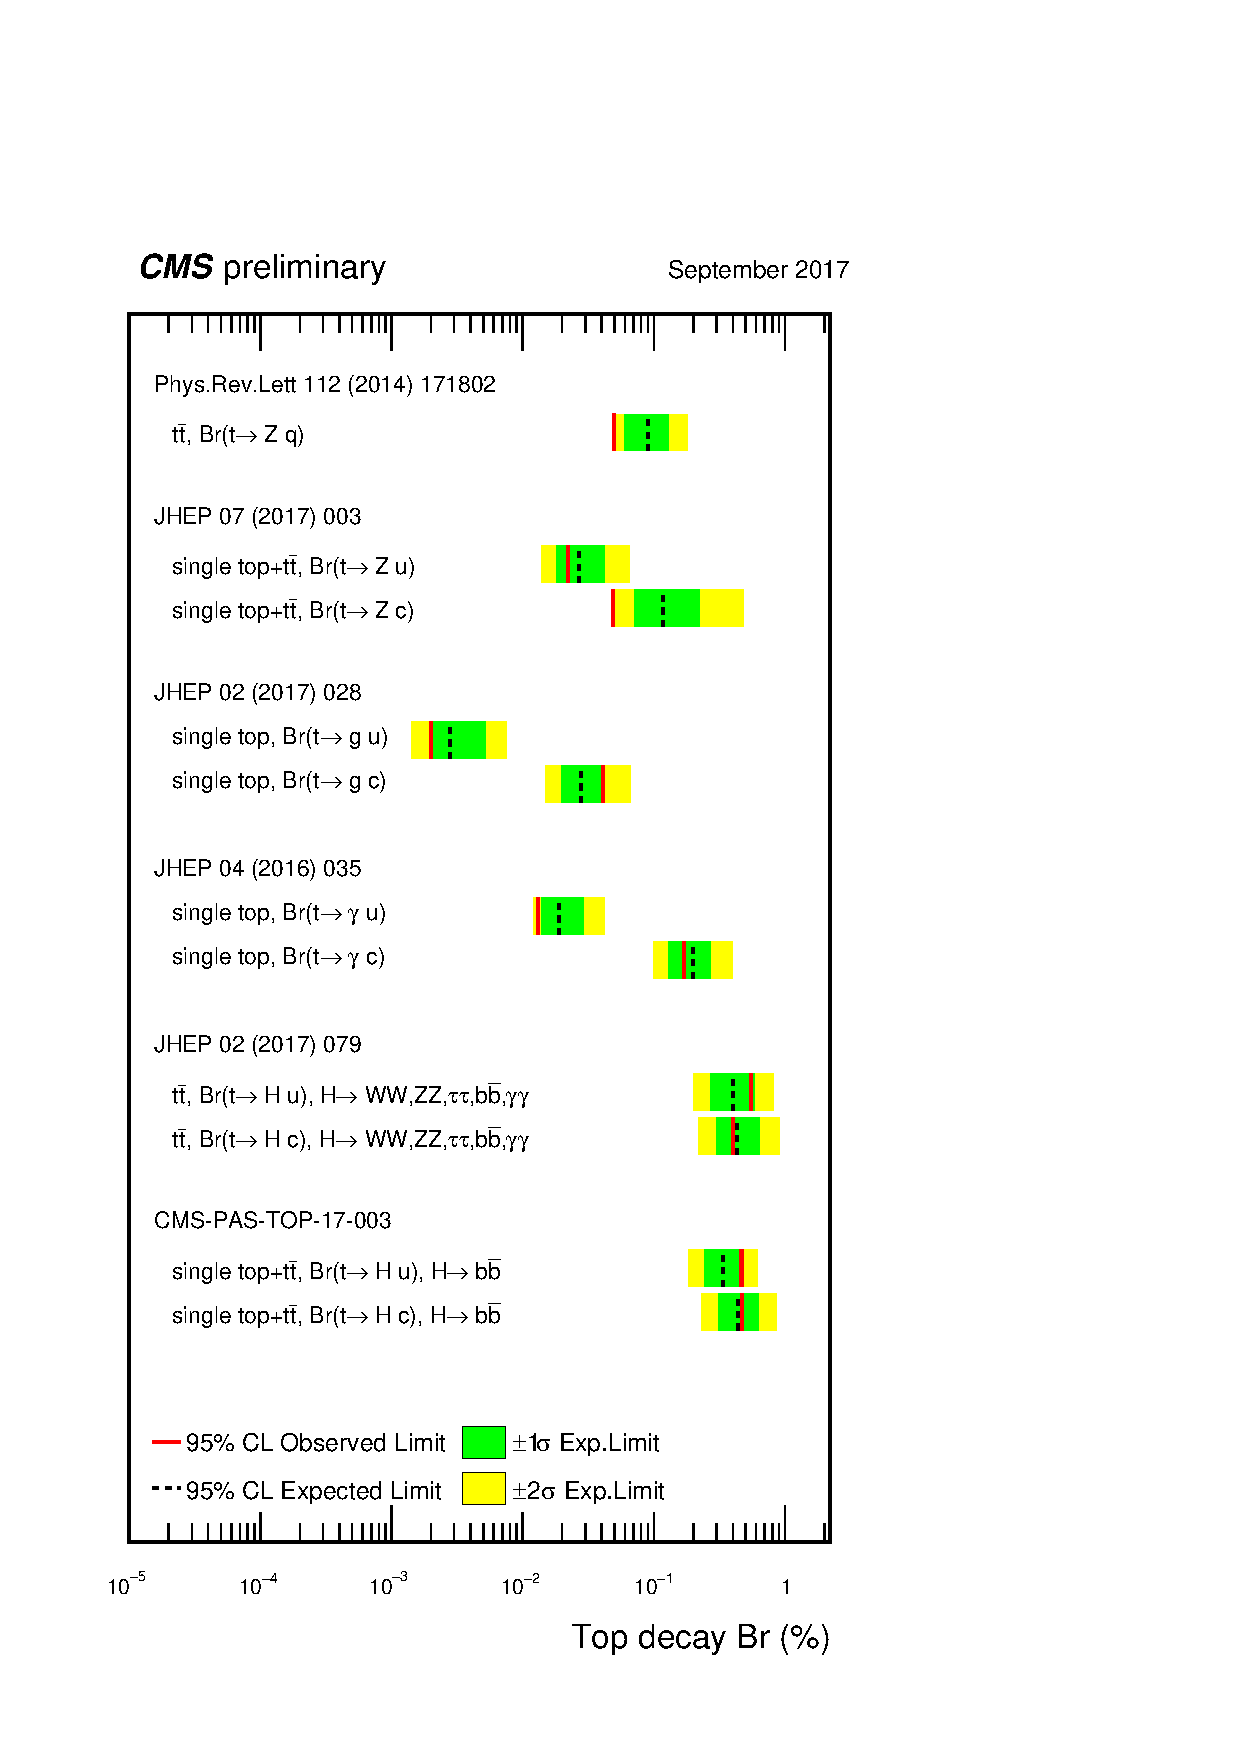
\includegraphics[width=0.7\linewidth]{1_Introduction/Figures/summary_FCNC.pdf}
	\caption{Summary of the FCNC branching fractions from CMS searches at a centre-of-mass energy of 8~\TeV. Figure taken from~\cite{summarywiki}.}
	\label{fig:summaryfcnc}
\end{figure}
\begin{figure}[htbp]
	\centering
	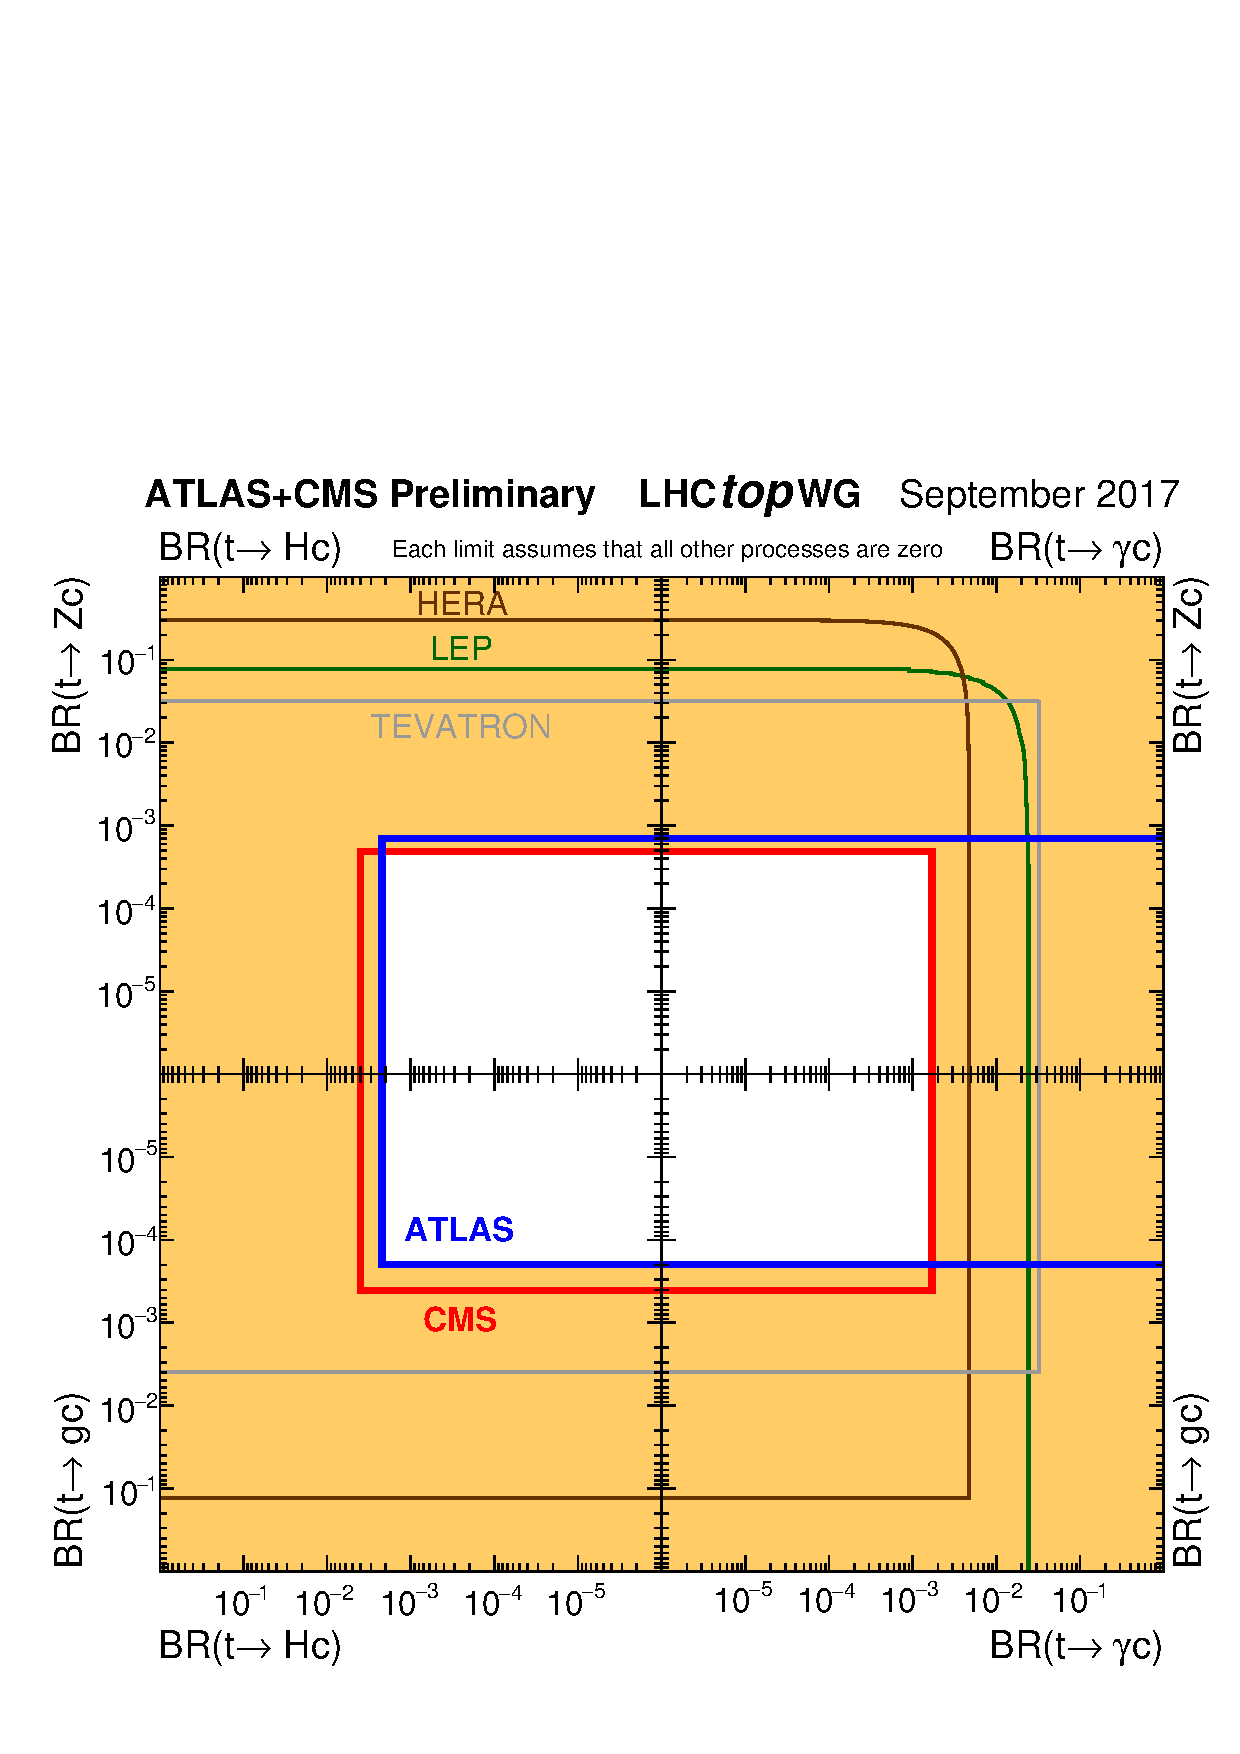
\includegraphics[width=0.49\linewidth]{1_Introduction/Figures/fcnc_tXc_sep17.pdf}
	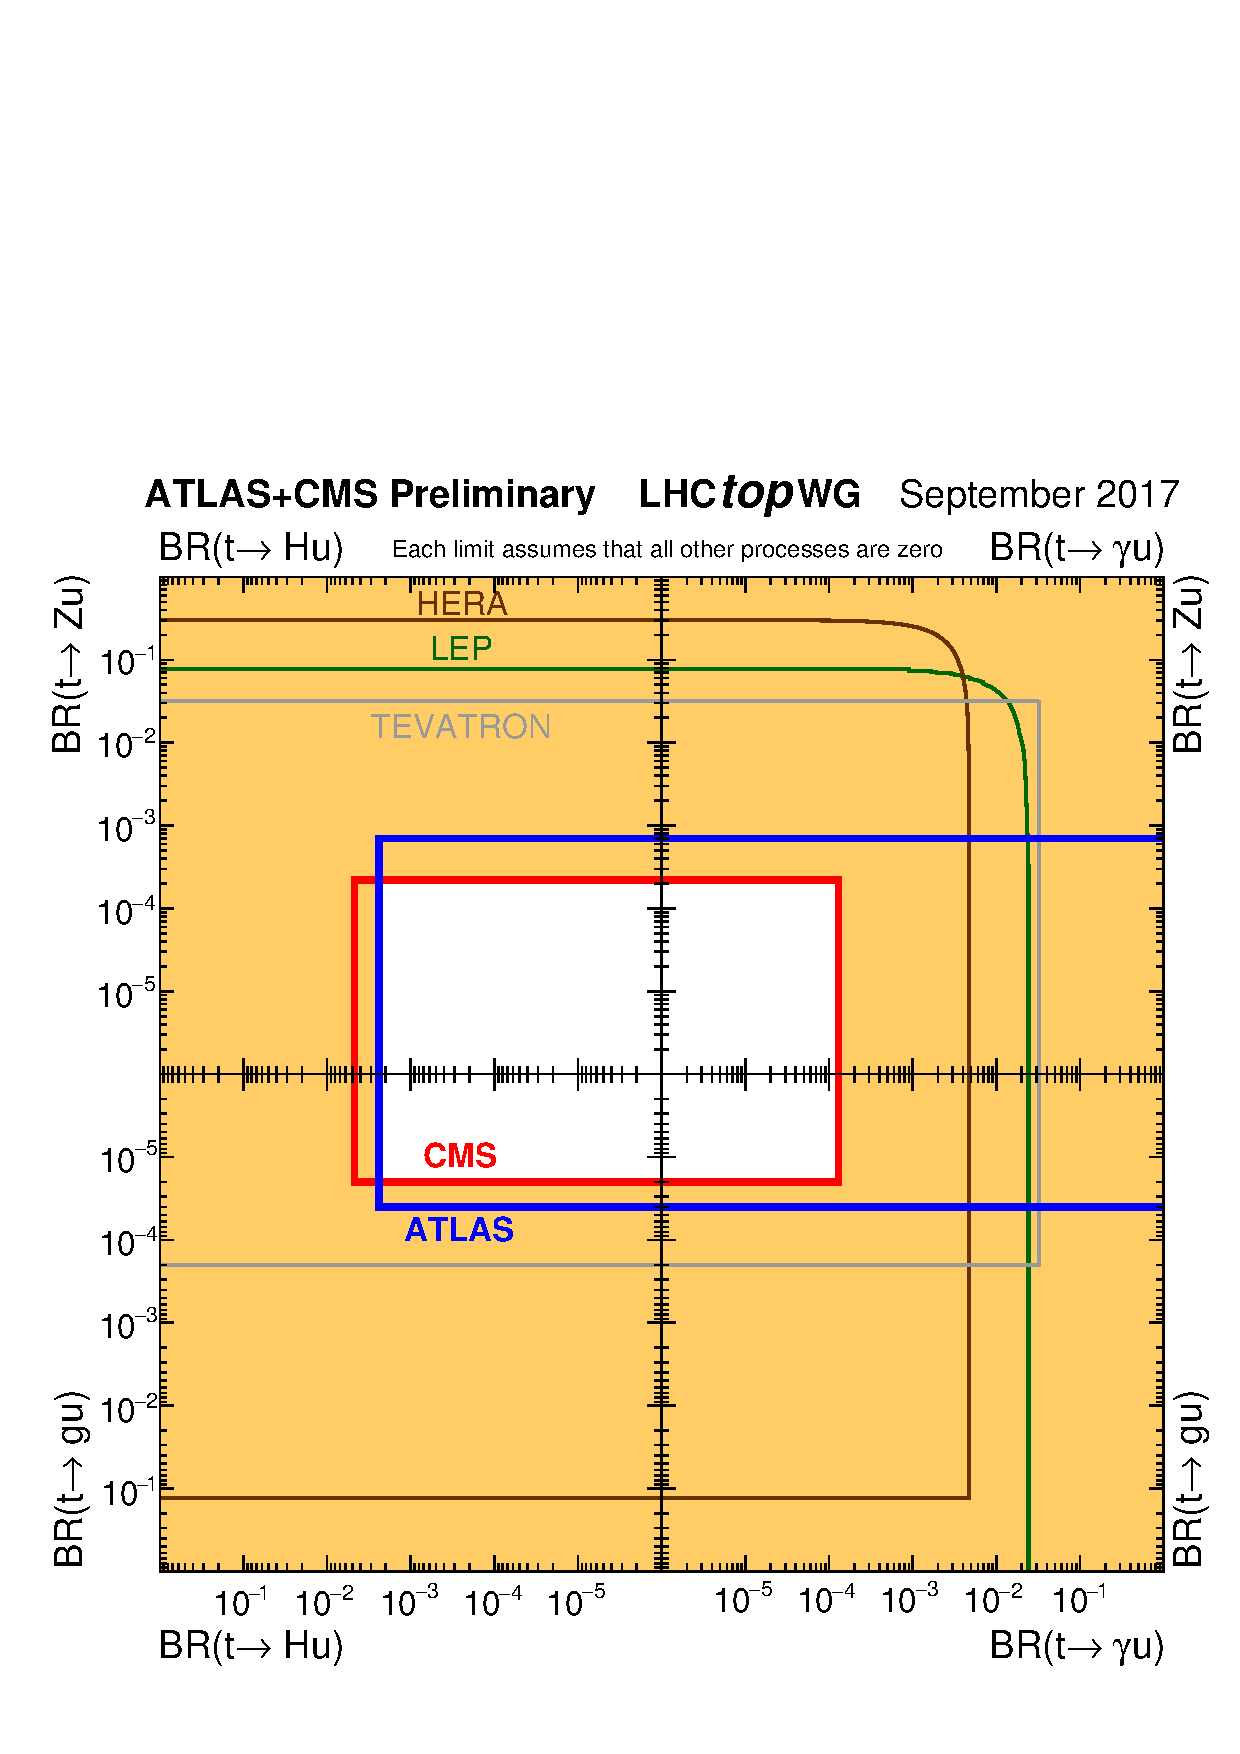
\includegraphics[width=0.49\linewidth]{1_Introduction/Figures/fcnc_tXu_sep17.pdf}
	\caption{Summary of the current 95\% confidence level observed limits on the branching fractions of the top quark decays via flavour changing neutral currents to a charm (left) or up (right) quark and a neutral boson. The coloured lines represent the results from HERA (the most stringent limits between the ones obtained by the H1 and ZEUS collaborations, in brown), LEP (combined ALEPH, DELPHI, L3 and OPAL collaborations result, in green), TEVATRON (the most stringent limits between the ones obtained by the CDF and D0 collaborations, in grey). The yellow area represents the region excluded by the ATLAS and the CMS Collaborations. Figure taken from~\cite{summarytwiki}.}
	\label{fig:FCNCATLASCMS}
\end{figure}





